\documentclass[a4paper,fleqn]{cas-dc}
\usepackage{amsmath,amssymb,amsfonts}
\usepackage{algorithmic}
\usepackage{algorithm}
\usepackage{graphicx}
\usepackage{textcomp}
\usepackage{xcolor}
\usepackage{bbm}
\usepackage{amsthm}
\usepackage[T1]{fontenc}
\usepackage{microtype}
\usepackage{adjustbox}
\usepackage{placeins}
\setlength{\emergencystretch}{3em}
\usepackage{xurl}
\hypersetup{hidelinks}
\usepackage[numbers,sort&compress]{natbib}
\usepackage{booktabs}
\usepackage{tabularx}
\usepackage{multirow}
\usepackage{array}
\theoremstyle{plain}
\newtheorem{theorem}{Theorem}
\newtheorem{proposition}{Proposition}
\newtheorem{assumption}{Assumption}
\newtheorem{lemma}{Lemma}
\theoremstyle{remark}
\newtheorem{remark}{Remark}
\theoremstyle{plain}
\newcommand{\theadcell}[1]{\shortstack[c]{#1}}
\newcommand{\theadmulti}[1]{\multirow{2}{*}[-0.8ex]{\theadcell{#1}}}
\newcommand{\datamulti}[1]{\multirow{2}{*}[-0.4ex]{#1}}

\usepackage[switch]{lineno}
% Do not print an empty ORCID note while author metadata is incomplete.
\ExplSyntaxOn
\cs_new_eq:NN \cas_original_printorcid: \printorcid
\RenewDocumentCommand\printorcid{}{\seq_if_empty:NF\g_stm_orcid_seq{\cas_original_printorcid:}}
\ExplSyntaxOff

\begin{document}
\shorttitle{Learning-Assist Adaptive MPC for Data Center Energy Management}
\shortauthors{Author information to be completed}
\title[mode=title]{Learning-Assist Adaptive Chance-Constrained MPC for Renewable-Integrated Data Center Energy Management}

% TODO: Replace with actual authors, affiliations, and corresponding-author email.
% The original IEEE file contained only sample author and funding information.
\author[1]{Author information to be completed}
\affiliation[1]{organization={Affiliation to be completed},country={}}
% \author[1]{Full Name\corref{cor1}}
% \ead{corresponding.author@example.org}
% \cortext[cor1]{Corresponding author.}
% \tnotetext[funding]{Add the verified funding statement here if applicable.}

\begin{abstract}
Renewable-integrated data centers must make real-time dispatch and workload scheduling decisions under volatile renewable supply, electricity prices, workload arrivals, and thermal constraints, making real-time energy management central to both operating cost and service reliability. This paper proposes a learning-assist adaptive model predictive control (MPC) framework for this online energy management problem under multi-source uncertainty. The controller integrates renewable dispatch, battery operation, deferrable workload scheduling, IT--cooling thermal dynamics, and chance-constrained closed-loop risk tracking within a receding-horizon formulation. To mitigate short-horizon suboptimality, a DP-inspired terminal value function is trained offline by a compact linear program and embedded online as a convex piecewise-linear approximation. To reduce closed-loop conservatism, a sliding-window adaptive chance-constraint update tracks recent empirical violation statistics and adjusts the relaxation margins online. Closed-loop simulations show that, among causal controllers, the proposed windowed scheme attains the smallest cost gap to the hindsight benchmark, the lowest service level agreement (SLA) unserved ratio, and the highest renewable utilization. Robustness tests under forecast quality variations and hyper parameter perturbations show that the cost and empirical violation rate remain within narrow bands.
\end{abstract}

\begin{keywords}
data centers \sep adaptive MPC \sep chance constraints \sep energy management \sep thermal safety \sep renewable energy
\end{keywords}
\maketitle
\linenumbers

\section{Introduction}\label{sec:introduction}
Driven by the rapid scaling of Artificial Intelligence (AI), cloud computing, and data intensive services, data centers (DCs) are becoming a fast growing contributor to global electricity demand. In its 2025 \emph{Energy and AI} report, the International Energy Agency (IEA) estimates that, as of 2024, indirect CO$_2$ emissions from data centers account for about 0.5\% of global fuel combustion CO$_2$ emissions and could rise to 1.0\%--1.4\% by 2030 across its Base and Lift-Off cases~\cite{iea2025_energy_ai}. Against this backdrop, hyperscale operators (e.g., Google) are accelerating carbon-free electricity strategies through renewable procurement and, where applicable, on-site generation, targeting 24/7 carbon-free energy matching for data center campuses~\cite{google2025_environmental_report}.

However, decarbonizing DC operation is not only a power supply substitution problem: Information Technology (IT) electricity is converted into heat and is constrained by thermal safety limits~\cite{tang2008_thermal_aware_scheduling}, so DC energy management must move beyond siloed IT-only or cooling-only optimization. Many existing studies simplify the IT--cooling coupling by (i) adopting fixed power-usage-effectiveness (PUE) surrogates~\cite{ding2026_multi_time_scale_market}, (ii) omitting explicit thermal limits~\cite{lechowicz2023_online_pause_resume}, or (iii) treating the IT load as exogenous~\cite{lazic2018_dc_cooling_mpc}. This motivates a unified framework that co-optimizes workload, cooling, and power supply decisions under uncertainty.

Data centers are also attractive demand response resources because deferrable workloads can shift demand over time~\cite{liu2013_dr_coincident_peak}. This flexibility is often coupled with on-site battery energy storage systems (ESSs), which yields a tightly coupled problem driven by prices, renewables, storage dynamics, and workload deadlines~\cite{yu2018_distributed_realtime_dcmg}. Because workload shifting also affects heat generation and cooling demand, online DC energy management becomes a constrained cross-layer decision problem under multi-source uncertainty~\cite{xie2025_low_carbon_workload_thermal}. This motivates examining how predictive scheduling, terminal energy valuation, and adaptive violation feedback can be coordinated within an online controller.

\section{Related Work}\label{sec:related_work}

From the perspective of online decision-making paradigms, existing methods for data center energy management can be categorized into four classes, as summarized in Table~\ref{tab:lit_summary}.

\begin{table*}[t]
\centering
\caption{Literature summary of online data center energy management methods.}
\label{tab:lit_summary}
\setlength{\tabcolsep}{3pt}
\renewcommand{\arraystretch}{0.97}
\fontsize{8}{9}\selectfont
\renewcommand{\tabularxcolumn}[1]{m{#1}}

\begin{tabularx}{\textwidth}{@{}
    c
    >{\centering\arraybackslash}m{0.14\textwidth}
    >{\centering\arraybackslash}m{0.14\textwidth}
    >{\centering\arraybackslash}m{0.14\textwidth}
    >{\centering\arraybackslash}m{0.20\textwidth}
    >{\centering\arraybackslash}X
@{}}
\toprule
\textbf{Ref.} & \textbf{Temporal flexibility} & \textbf{Thermal awareness} & \textbf{Uncertainty Source} & \textbf{Model} & \textbf{Solution} \\
\midrule
\cite{lechowicz2023_online_pause_resume} & Hard (job-level) & -- & CI & Online policy & Threshold (analytic) \\
\cite{hanafy2023_carbonscaler} & Hard (job-level) & -- & IT, CI & Online policy & Greedy (analytic) \\
\midrule
\cite{xie2025_low_carbon_workload_thermal} & Soft (relaxed) & Hard safety limit & IT, Price, CI, Env & Lyapunov optimization & LP \\
\cite{gao2024_online_electricity_dvb} & Hard (aggregated) & Hard safety limit & IT, RES, Price, Env & Lyapunov optimization & Lyapunov online optimization \\
\midrule
\cite{chakraborty2025_renewable_overbooking} & -- & -- & IT, RES & MDP (discrete-time) & Value iteration \\
\cite{chitsaz2024_ctmdp_power_mgmt} & Only queue model & -- & IT & MDP (continuous-time) & Iterative DP \\
\cite{ding2026_multi_time_scale_market} & Soft (delay penalty) & -- & IT, Price & DRL (DDPG) & Actor--critic \\
\cite{ding2025_job_scheduling_uncertain} & Hard (job-level) & -- & IT, Price & Distributional RL & QR-DQN (CVaR) \\
\cite{zhan2025_cooling_offline_rl} & -- & Thermal penalty & IT & Offline RL & TD3+BC-based \\
\cite{zhao2025_rl_holistic_energy} & -- & Thermal penalty & IT, RES & DRL (BayesDDQN) & DDQN + Bayesian opt. \\
\cite{ran2026_d3t_dual_timescale} & Soft (delay penalty) & Thermal penalty & IT, RES, Price & Dual-timescale DRL & DQN + QMIX \\
\cite{chi2021_multi_agent_drl_efficiency} & Soft (delay penalty) & Thermal penalty\textsuperscript{*} & IT & Multi-agent DRL & Actor--critic \\
\cite{jin2022_optimal_policy_ppo} & Soft (delay penalty) & -- & IT, RES & DRL (PPO) & Policy gradient \\
\midrule
\cite{guo2024_multitimescale_mpc_interconnected_dcs} & Hard (class deadlines) & Hard safety limit & IT, RES, Env & Multi-timescale MPC & ADMM \\
\cite{wang2025_mpc_cooling_workload_rack_dc} & -- & Soft safety limit & IT & State-space MPC & SQP \\
\cite{zhu2022_smpc_dcmg_dispatch} & Hard (aggregated) & -- & IT, RES & Stochastic MPC & MILP \\
\cite{li2024_robust_mpc_thermal_rack} & -- & Hard safety limit & IT, Env & Robust MPC & NLP \\
\cite{li2023_subspace_mpc_air_cooled} & -- & Hard safety limit & -- & Subspace MPC & SQP \\
\cite{lazic2018_dc_cooling_mpc} & -- & Thermal penalty & IT, Env & Deterministic MPC & Gradient-based (Adam) \\
\midrule
\textbf{Proposed} & Hard (full flexibility) & Chance constraint & IT, RES, Price, Env & Learning-assist MPC & offline LP + online LP \\
\bottomrule
\end{tabularx}

\vspace{0.15em}
\begin{minipage}{\textwidth}
\fontsize{8}{9}\selectfont
\raggedright
\textit{Notes:}
IT = IT workload/power; RES = renewable energy sources; CI = carbon intensity; Price = electricity price; Env = external thermal conditions. Listed inputs need not have explicit forecast-error models. In this work, Env is treated as an available exogenous input, not as a forecast error source.
DP = dynamic programming; ADMM = alternating direction method of multipliers; LP/NLP/SQP = linear/nonlinear/sequential quadratic programming; MILP = mixed-integer linear programming.
``Hard'' denotes hard deadline constraints for deferrable workloads; ``Soft'' denotes either time-average relaxed constraints (virtual queues) or delay-penalty costs in the objective; temporal flexibility labels describe deferrable workload modeling.
``Job-level'' denotes an explicit completion deadline for each deferrable job; ``Full flexibility'' means real-time arrivals with heterogeneous per job deadlines; ``Class deadlines'' denotes workload classes with maximum delay constraints; ``Aggregated'' means an aggregate deferrable demand/queue model; ``Only queue model'' indicates an aggregated queue without per job deadlines.
For thermal awareness, ``Hard safety limit'' enforces deterministic safety bounds; ``Soft safety limit'' uses relaxed temperature bounds or violation penalties; ``Chance constraint'' denotes a specified violation-risk target; ``Thermal penalty'' means thermal effects are handled via an objective penalty. \textsuperscript{*}\cite{chi2021_multi_agent_drl_efficiency} also uses an overheating protector.
\end{minipage}

\end{table*}

(i) \textit{Deterministic online scheduling.}
Methods in this category make slot-by-slot decisions using revealed information or point forecasts. Hanafy et al.~\cite{hanafy2023_carbonscaler} develop a marginal-gain greedy rule for scheduling deferrable workloads under low-carbon operation; however, its performance depends on forecast quality. Lechowicz et al.~\cite{lechowicz2023_online_pause_resume} formulate an online pause-and-resume model that yields a two-threshold policy with competitive guarantees under switching costs. Nevertheless, their simplified action structures (e.g., run/pause switching or threshold rules) cannot easily represent general continuous controls coupled with explicit thermal constraints (Table~\ref{tab:lit_summary}).

(ii) \textit{Online virtual queue management (Lyapunov optimization).}
Lyapunov controllers make per slot decisions through virtual queues and time-average objectives, often without requiring prior statistical knowledge or forecasts~\cite{xie2025_low_carbon_workload_thermal,gao2024_online_electricity_dvb}. These controllers combine time-average optimization with parameter-dependent feasibility guarantees. Their queue-based formulations differ from the explicit arrival-group scheduling and recent-window violation feedback considered here. Capturing such intertemporal coupling and forecast feedback motivates forward looking modeling that leads to MDP-based formulations.

(iii) \textit{Markov decision process (MDP)-based sequential decision-making.} This class includes model-based dynamic programming (DP) and data-driven reinforcement learning (RL), including its deep variants (DRL). Model-based DP offers interpretability and explicit constraint modeling; however, when the environment is time-varying or cannot be modeled with high fidelity, model mismatch may accumulate over multi-step rollouts and degrade long run performance~\cite{chakraborty2025_renewable_overbooking,chitsaz2024_ctmdp_power_mgmt}. RL learns policies or value functions from data and has been increasingly applied to DC IT--cooling coordination and workload scheduling~\cite{zhao2025_rl_holistic_energy,ran2026_d3t_dual_timescale,ding2025_job_scheduling_uncertain}. Despite these advances, RL-based controllers in safety critical DC operations often handle thermal limits through reward penalties, sometimes with additional safeguards, require substantial training data, and rely on large scale nonconvex optimization with limited convergence guarantees. This motivates an MPC backbone that imposes explicit constraints and tracks closed-loop risk.

(iv) \textit{MPC with receding-horizon optimization.}
MPC explicitly models operational constraints and, at each time step, updates predictions and solves a finite-horizon optimization problem. It is widely adopted in engineering practice for interpretable online dispatch, cooling system control, and workload--thermal co-optimization~\cite{guo2024_multitimescale_mpc_interconnected_dcs,zhu2022_smpc_dcmg_dispatch,wang2025_mpc_cooling_workload_rack_dc,li2024_robust_mpc_thermal_rack,li2023_subspace_mpc_air_cooled}. Nevertheless, existing DC-oriented MPC studies usually focus on cooling side dispatch, aggregate demand models, or deterministic safety bounds or penalty-based thermal handling. They rarely combine heterogeneous per job deferrable workload scheduling with adaptive closed-loop thermal-risk tracking under forecast errors (Table~\ref{tab:lit_summary}).

Within MPC, uncertainty handling determines the tradeoff between cost and feasibility. Robust MPC, including tube-based formulations, does not require an explicit probability distribution but relies on a priori bounded uncertainty sets, which can be conservative and difficult to specify under multi-source uncertainty~\cite{singh2016_tube_mpc_contraction}. Chance-constrained stochastic MPC (CC-SMPC) explicitly balances performance and constraint satisfaction, but conventional pointwise chance constraints can be overly conservative in closed-loop operation~\cite{oldewurtel2013_adaptive_cc_smpc}. To address this, Ghosh et al.~\cite{ghosh2025_adaptive_relaxation_ccsmpc} update the relaxation margin from observed violations; building on this idea, we adopt a sliding-window estimator that emphasizes recent risk and provide a convergence analysis to the target violation level under standard assumptions.

Besides constraint and risk handling, the long run performance of MPC also depends on the terminal cost approximation. Incorporating a terminal cost is a classical MPC technique that connects finite-horizon objectives with long run performance, serving as a surrogate for beyond-horizon behavior~\cite{mayne2000_constrained_mpc}. Rather than relying on hand-crafted terminal penalties or on horizon extension (which amplifies forecast errors), we learn a DP-inspired terminal value function offline through a compact linear program, and embed its convex piecewise-linear approximation into the MPC objective.

Most of the related work above concerns single data center energy management. Although geo-distributed coordination is an active research area~\cite{souza2024_casper_carbon_aware,maji2023_carbon_multicloud}, cross-site scheduling must account for transmission delays~\cite{li2021_joint_energy_compute} and, when coordinating multiple service providers, operational privacy~\cite{sun2025_privacy_energy_sharing}. This paper focuses on single data center online energy management as a necessary first step toward scalable multi-site coordination. The main contributions are summarized as follows.
\begin{enumerate}
\item Unlike existing DC-oriented MPC studies that typically focus on cooling-side dispatch, aggregated demand models, or non-probabilistic thermal handling (Table~\ref{tab:lit_summary}), we develop a unified online MPC framework that simultaneously integrates heterogeneous deferrable workload scheduling, IT--cooling thermal coupling, ESS dynamics, and chance-constrained closed-loop risk tracking under data-driven forecast errors.

\item We propose a sliding-window adaptive chance-constraint update that extends the time-average mechanism of~\cite{ghosh2025_adaptive_relaxation_ccsmpc} by tracking the empirical violation rate over a recent window, emphasizing recent risk dynamics rather than the full history. We further characterize closed-loop target tracking: under an ideal one-step controllability assumption the windowed empirical violation rate converges to the target $\alpha_i$ up to the residual induced by the finite window length, and under a weaker attainability assumption the update is one-step optimal and admits a structural performance envelope of order $1/\sqrt{w}$ around the projected target.

\item We obtain a DP-inspired terminal value function from a compact LP reformulation of the Bellman recursion and embed it into the MPC objective as a convex piecewise-linear surrogate of the long term cost-to-go. Unlike hand-crafted terminal penalties, horizon extension (which amplifies forecast errors), or RL-based value network learning, this construction yields a tractable convex terminal value without hand-crafted terminal penalty tuning or nonconvex value network training.
\end{enumerate}

These contributions are empirically evaluated in Section~\ref{sec:case_studies} through five year closed-loop simulations under multi-source uncertainty, component-wise ablation, risk-target sweeps, and LSTM-residual and hyper-parameter sensitivity studies. The remainder of the paper is organized as follows. Section~\ref{sec:modeling} presents the data center modeling framework, Section~\ref{sec:offline_training} introduces the offline terminal-value training procedure, and Section~\ref{sec:adaptive_mpc} develops the adaptive chance-constrained MPC formulation and implementation details. Section~\ref{sec:case_studies} reports the case studies, Section~\ref{sec:conclusion} concludes the paper, and the detailed proofs are given in the Appendix.


\section{Data Center Modeling}\label{sec:modeling}
Fig.~\ref{fig:system_architecture_overview} provides a overview of the single data center architecture considered here. It highlights the electrical supply side, the IT workload execution side, and the cooling subsystem; the component-level models are introduced in the following subsections.

\begin{figure*}[t]
\centering
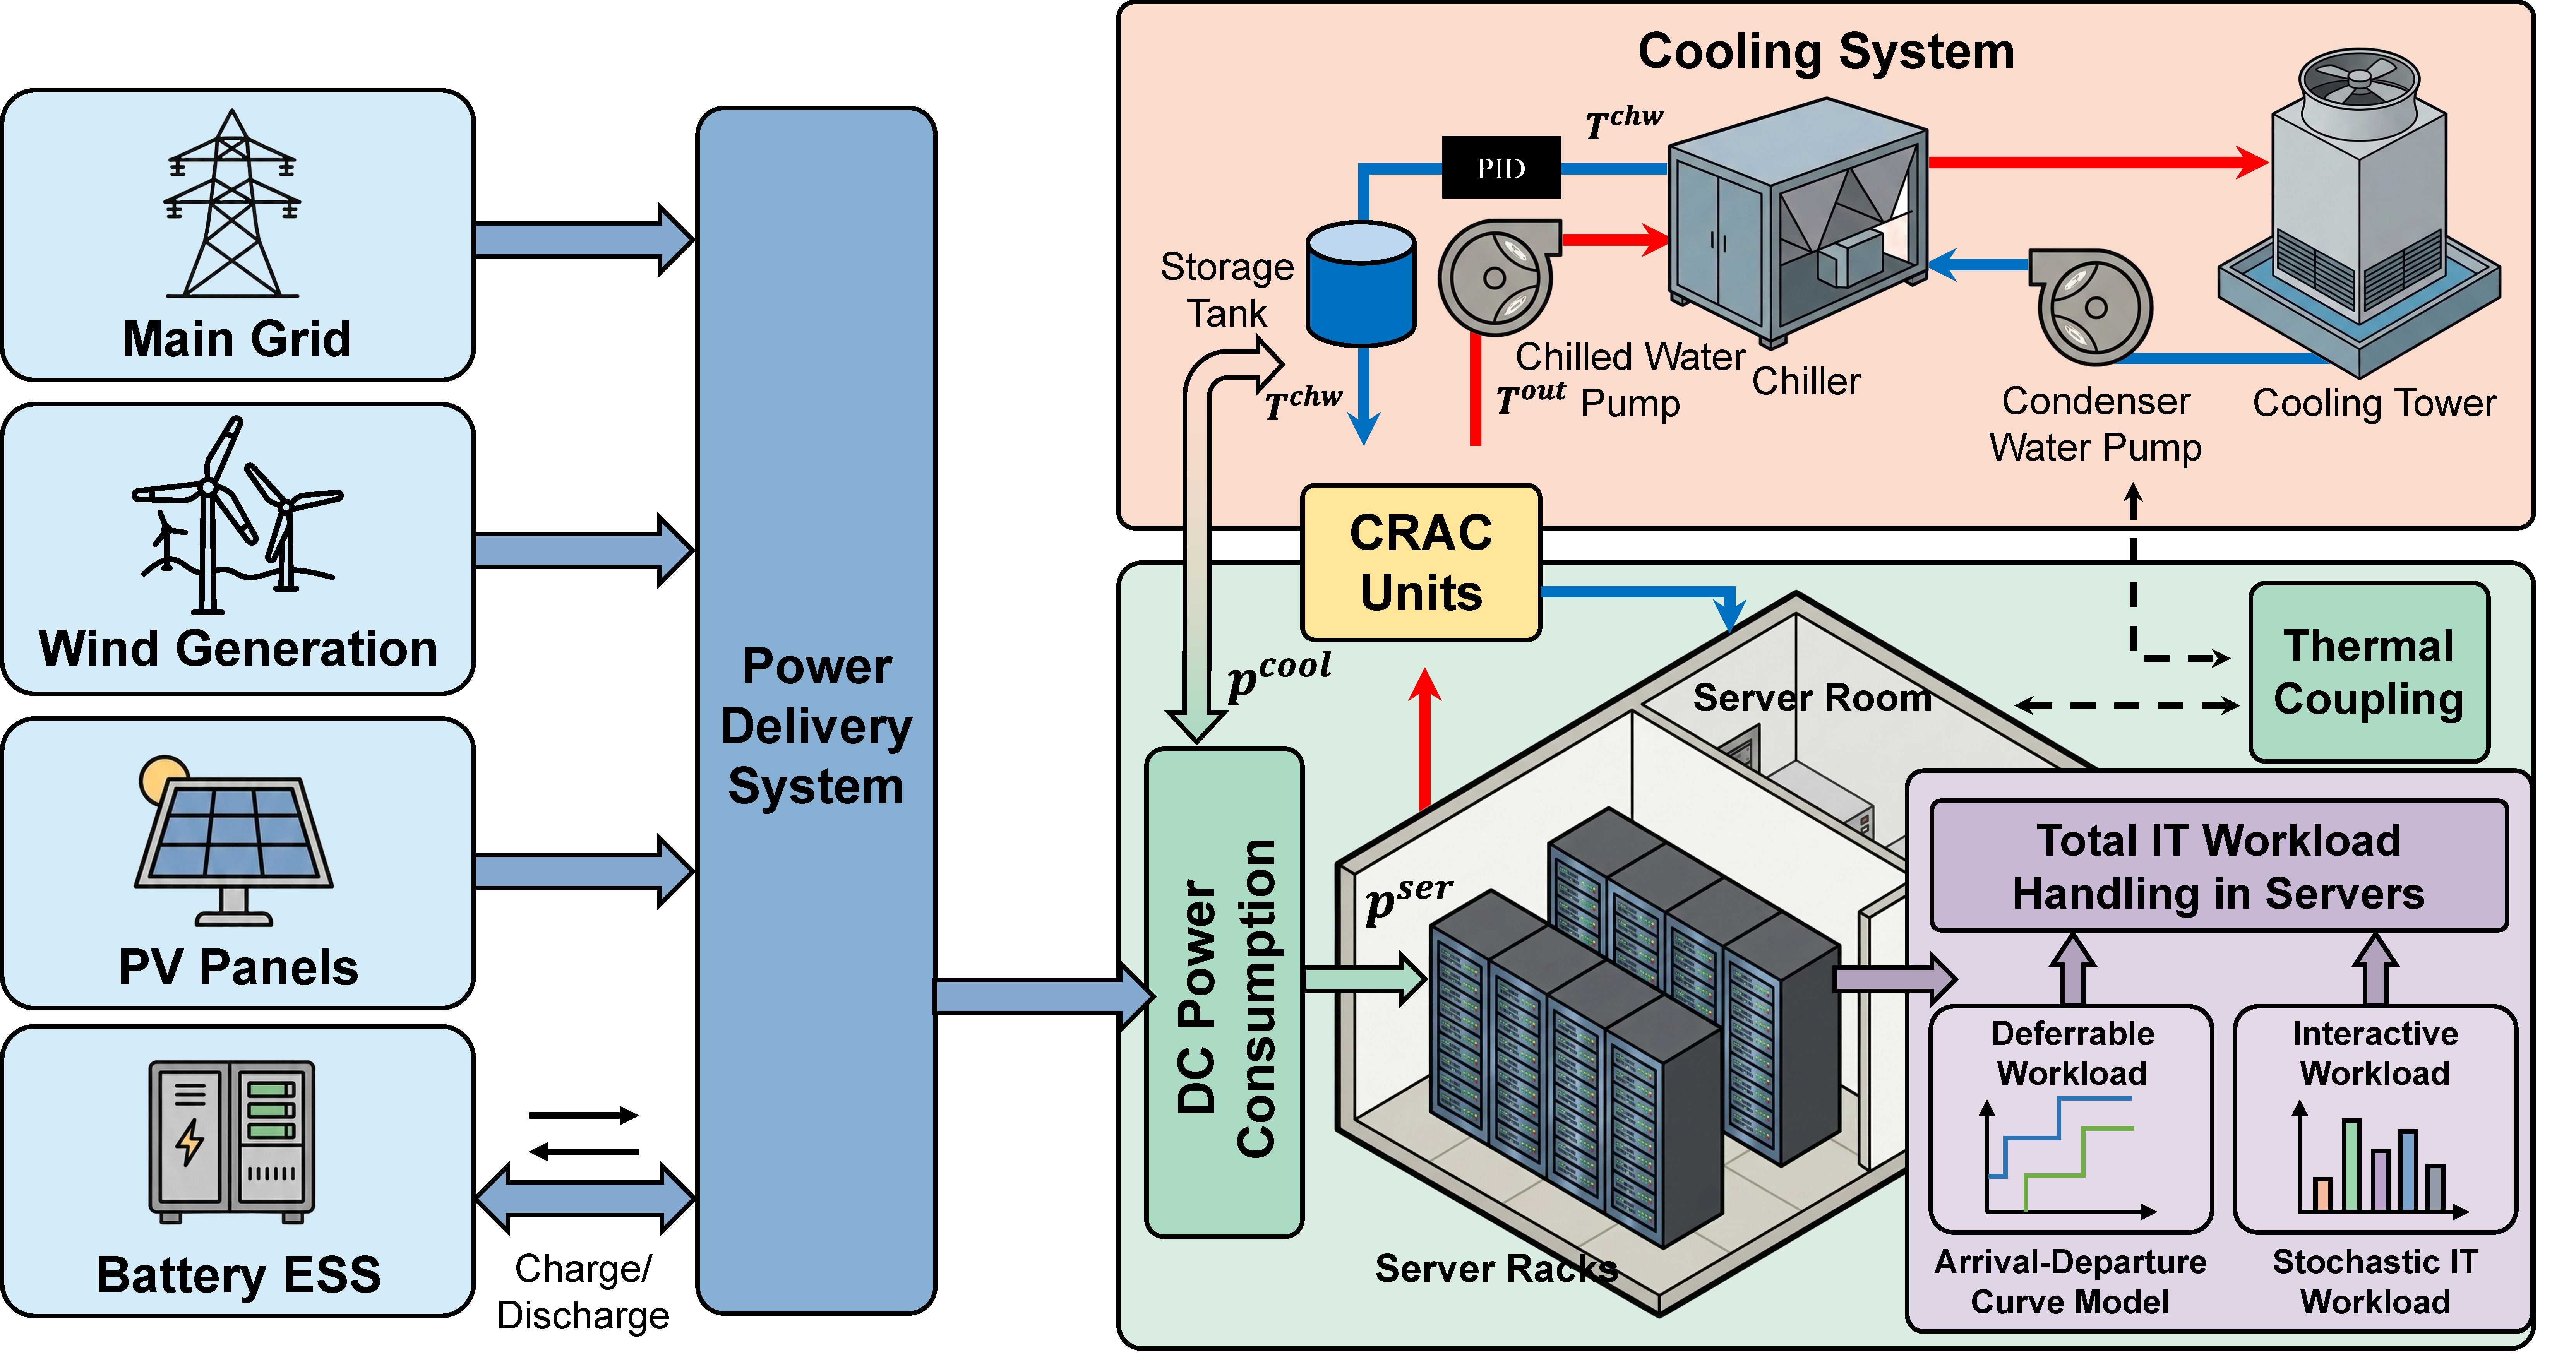
\includegraphics[width=\textwidth,height=0.72\textheight,keepaspectratio]{fig_system_arch/system_architecture.pdf}
\caption{System architecture of the studied single data center.}
\label{fig:system_architecture_overview}
\end{figure*}

\subsection{Workload Model}
User requests are submitted to the DC, assigned to internal IT resources for processing, and returned after completion. According to their time sensitivity, workloads are classified as interactive or deferrable. For deferrable workloads, service level agreement (SLA) requirements are satisfied provided that the tasks are completed within the prescribed time window. Since this paper addresses the real-time dispatch problem of a single DC, only the temporal flexibility of deferrable loads is modeled; the model is detailed below.

Fig.~\ref{fig:deferrable_workload_model} illustrates the deferrable workload abstraction.
Deferrable arrivals are grouped by release time and SLA class, scheduled within their admissible deadline windows, and aggregated into the slot-level executed deferrable workload that feeds the IT power model. Here, $A(t)$ denotes the cumulative deferrable workload arrivals up to slot $t$, $D(t)$ the cumulative executed deferrable workload, and $D_{\min}(t)$ the minimum cumulative service required by slot $t$ to satisfy all active deadlines~\cite{li2023_dcmg_balanced_decision}.

\begin{figure*}[t]
\centering
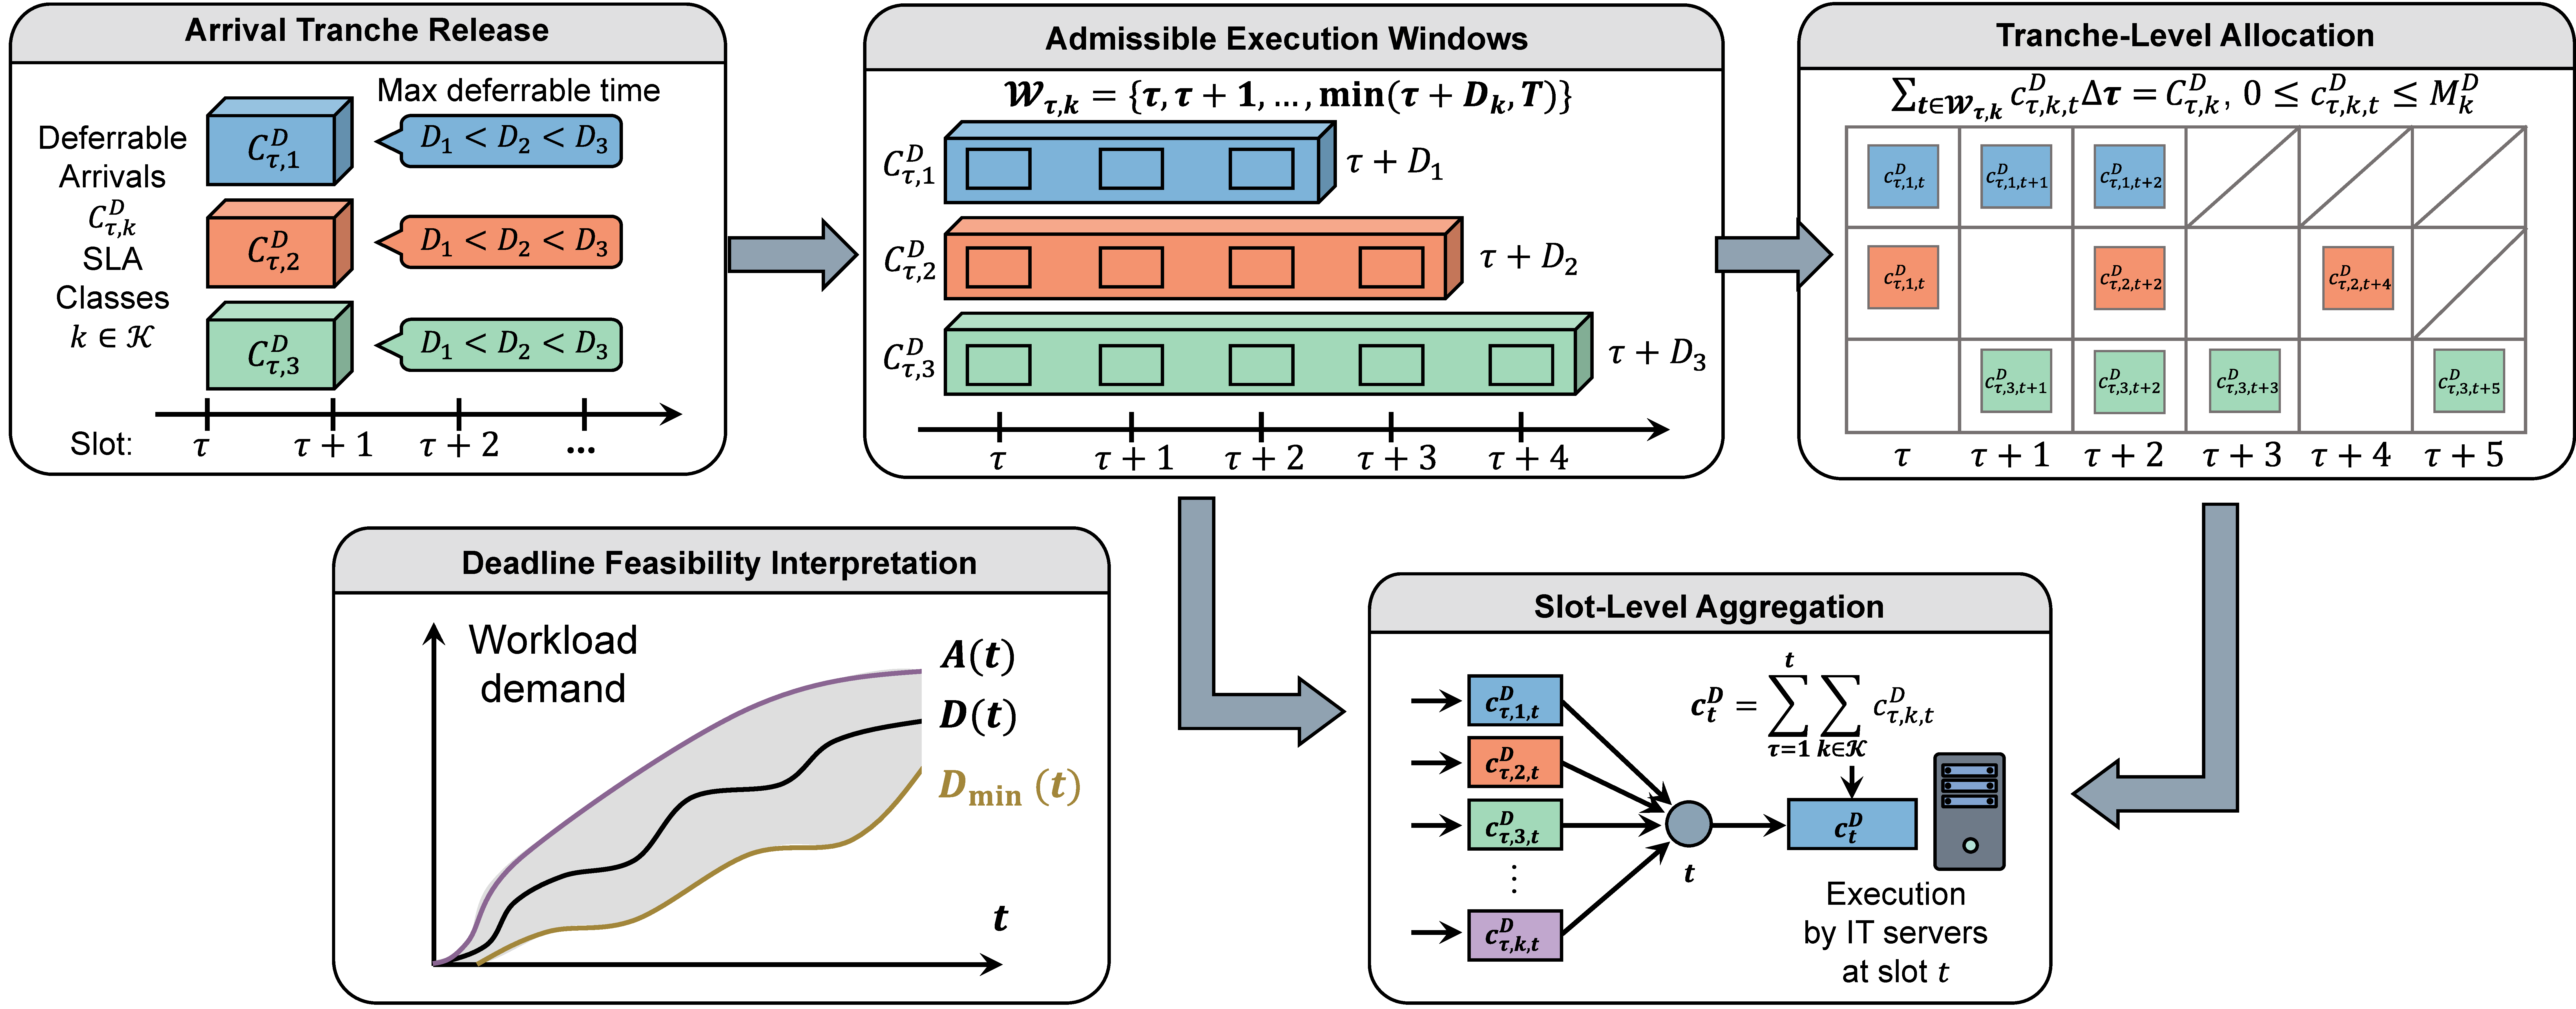
\includegraphics[width=\textwidth,height=0.72\textheight,keepaspectratio]{fig_workload_model/deferrable_workload_explanation_update.pdf}
\caption{Illustration of the deferrable workload model. Deferrable arrivals are grouped by release time and SLA class, allocated within their admissible execution windows, and aggregated into the slot-level deferrable CPU utilization. The cumulative curves $A(t)$, $D(t)$, and $D_{\min}(t)$ show arrivals, executed workload, and the minimum service required to meet active deadlines.}
\label{fig:deferrable_workload_model}
\end{figure*}

To capture heterogeneous deferrable workloads under different SLAs, we group deferrable demand by release time and SLA class.
Let $\mathcal{K}$ denote the set of deferrable workload classes. Each class $k\in\mathcal{K}$
is characterized by a maximum deferral (deadline) $D_k$ and a per-slot CPU allocation limit $M_k^D$.
At each arrival slot $\tau\in\{1,\ldots,T\}$, the incoming deferrable demand is represented by
$\{C_{\tau,k}^D\}_{k\in\mathcal{K}}$, where $C_{\tau,k}^D$ is the total normalized CPU-time demand (e.g., core$\cdot$slot)
assigned to class $k$ and released at slot $\tau$. Each pair $(\tau,k)$ defines an arrival group.

We define $c_{\tau,k,t}^D$ as the CPU resources allocated at execution slot $t$ to serve the deferrable demand
in arrival group $(\tau,k)$, and $T$ denotes the total number of time slots in a day. Let $\mathcal{T}:=\{1,\ldots,T\}$ and define the admissible execution window
$\mathcal{W}_{\tau,k}:=\{\tau,\tau+1,\ldots,\min(\tau+D_k,T)\}$ for each $(\tau,k)\in\mathcal{T}\times\mathcal{K}$.
The deferrable deadline constraints are:
\begin{equation}\label{eq:pd}
\sum_{t\in \mathcal{W}_{\tau,k}} c_{\tau,k,t}^D \,\Delta\tau = C_{\tau,k}^D,
\quad \forall (\tau,k)\in \mathcal{T}\times\mathcal{K}.
\end{equation}
\begin{equation}\label{eq:bounds}
0 \le c_{\tau,k,t}^D \le M_k^D,
\quad \forall (\tau,k)\in \mathcal{T}\times\mathcal{K},\ \forall t\in \mathcal{W}_{\tau,k}.
\end{equation}
Let $\Delta\tau$ denote the length of one discrete time slot. The total deferrable CPU utilization executed at slot $t$ is the aggregation of all active time slots:
\begin{equation}\label{eq:pd_agg}
c_t^D = \sum_{\tau=1}^{t}\sum_{k\in\mathcal{K}} c_{\tau,k,t}^D,\quad \forall t \in \mathcal{T}.
\end{equation}


IT equipment in a DC is heterogeneous, in the sense that hardware parameters vary across devices. In addition, each incoming task is subject to resource limits (e.g., CPU and memory), which increases the complexity of the scheduling problem. Radovanovic et al.~\cite{radovanovic2023_carbon_aware_computing} show that CPU usage alone provides an accurate proxy for power consumption across Google power domains, and that this conclusion holds in heterogeneous hardware environments. For tractability, we approximate IT server power as an affine function of CPU utilization:
\begin{equation} \label{eq:pser}
p_t^{\text{ser}} = (p_{\max}^{\text{ser}}-p_{\text{idle}}^{\text{ser}})\cdot u_t + p_{\text{idle}}^{\text{ser}}, \quad \forall t\in\mathcal{T}.
\end{equation}
\begin{equation}\label{eq:util}
u_t = \frac{c_t^I + c_t^D}{c^M}, \quad \forall t\in\mathcal{T}.
\end{equation}
\begin{equation}\label{eq:cap}
0 \le c_t^D + c_t^I \le c^M ,\quad \forall t\in\mathcal{T}.
\end{equation}
where $p_{\text{idle}}^{\text{ser}}$ and $p_{\max}^{\text{ser}}$ represent the idle and peak power of IT servers, respectively. $u_t \in \left[0, 1\right]$ is the CPU utilization rate, $c_t^I$ denotes the CPU resources required by interactive workloads, $c_t^D$ is the total deferrable CPU executed at slot $t$ defined in \eqref{eq:pd_agg}, and $c^M$ denotes the CPU resource capacity of the DC.

In \eqref{eq:pser}, only the CPU utilization $u_t$ is treated as a control variable. Related studies consider cross-server workload redistribution~\cite{li2023_thermal_aware_failure} and optimize server activation to reduce idle power consumption~\cite{chitsaz2024_ctmdp_power_mgmt}. Such approaches introduce integer on/off decisions and startup dynamics, which increase the control problem's complexity. In production environments such as Google, all available machines in the DC are typically kept powered on unless they are damaged~\cite{radovanovic2023_carbon_aware_computing}.

\subsection{Cooling System Model}
The data center considered here uses room air cooling through computer room air conditioning (CRAC) units supported by a chilled water loop, as shown in Fig.~\ref{fig:system_architecture_overview}. The CRAC units remove heat from the server room, while the chilled water loop, chiller, pumps, and cooling tower reject the heat to the outdoor environment. The chilled water supply temperature $T_t^{\text{chw}}$ is used as the supervisory cooling setpoint and tracked by a local PID loop.

The total cooling system power is modeled by an aggregate linear surrogate that depends on the IT power consumption and the chilled water supply temperature. The surrogate captures the combined effects of chillers, pumps, cooling towers, and auxiliary devices while remaining linear and suitable for online optimization:
\begin{equation}\label{eq:Cooling}
p_t^{\text{cool}}
=c_t^{\text{1,env}} \cdot p_t^{\text{ser}}
+c_t^{\text{2,env}} \cdot T_t^{\text{chw}}
+c_{\text{3}}, \quad \forall t\in\mathcal{T}.
\end{equation}

Here, $p_t^{\text{cool}}$ denotes the total cooling system power consumption at slot $t$,
$p_t^{\text{ser}}$ is the IT/server power, and $T_t^{\text{chw}}$ is the chilled water supply temperature.
$c_{\text{3}}$ represents an aggregate base load, while $c_t^{\text{1,env}}$ and $c_t^{\text{2,env}}$
are environment-dependent coefficients. 

The influence of the external environment on the efficiency of the cooling system is described in \eqref{eq:env},
where $T_t^{\text{env}}$ and $H_t^{\text{env}}$ are the external environmental temperature and humidity, respectively. The coefficients $f_1,\ldots,f_6$ are fitted parameters of the linear cooling equation.
\begin{equation}\label{eq:env}
\left\{\begin{array}{l}
c_t^{\text{1,env}}=f_1 \cdot T_t^{\text{env}}+f_2 \cdot H_t^{\text{env}}+f_3, \quad \forall t\in\mathcal{T} \\
c_t^{\text{2,env}}=f_4 \cdot T_t^{\text{env}}+f_5 \cdot H_t^{\text{env}}+f_6, \quad \forall t\in\mathcal{T}
\end{array}\right.
\end{equation}
Ambient temperature and humidity affect cooling efficiency, but their forecast errors are difficult to characterize accurately. In the closed-loop simulations, they are treated as measured inputs over the short horizon. The remaining thermal deviations are managed through the receding horizon update, the thermal safety constraints, and the feasibility correction applied to the realized trajectory.

The server rack outlet air temperature $T_t^{\text{out}}$ is bounded by its maximum allowable value $T_{\max}^{\text{out}}$:
\begin{equation}\label{eq:T_temp}
    T_t^{\text{out}} \leq T_{\max }^{\text{out}}, \quad \forall t \in \mathcal{T}.
\end{equation}
The chilled water supply setpoint is constrained to the interval $[T_{\min}^{\text{chw}},T_{\max}^{\text{chw}}]$. For analytical tractability, the outlet air temperature dynamics are modeled as a linear function:
\begin{equation}\label{eq:Tchw}
\begin{aligned}
T_{\min }^{\text{chw}} & \leq T_t^{\text{chw}} \leq T_{\max }^{\text{chw}}, \quad \forall t\in\mathcal{T} \\
-\zeta \Delta \tau & \leq T_{t+1}^{\text{chw}}-T_{t}^{\text{chw}} \leq \zeta \Delta \tau, \quad \forall t\in\mathcal{T} \\
T_{t+1}^{\text{out}}& =T_{t}^{\text{out}} + d_1 \cdot p_t^{\text{ser}}+d_2 \cdot T_t^{\text{chw}}, \quad \forall t\in\mathcal{T}
\end{aligned}
\end{equation}
where $p^{\text{ser}}_{t}$ is the IT power, $T_t^{\text{chw}}$ is the chilled water supply setpoint, $\zeta$ denotes the maximum allowable rate of change for these temperatures, and $d_1,d_2$ are parameters of the linear outlet air temperature model.



\subsection{Generation Side Modeling}\label{subsec:gener}

The energy storage system (ESS) is characterized by the power limit $P_{\max}^{bs}$ and the nominal energy bounds $E_{\min}^{bs}$ and $E_{\max}^{bs}$. The corresponding constraints are expressed in \eqref{eq:Ebs}:
\begin{subequations}\label{eq:Ebs}
\begin{align}
E_{t+1}^{bs}
&=E_{t}^{bs}
+\!\left(
\eta_{\text{ch}}\, p_{t}^{\text{ch}}
-\frac{1}{\eta_{\text{dis}}}\, p_{t}^{\text{dis}}
\right)\Delta \tau, \forall t \in \mathcal{T},
\\
-P_{\max }^{bs}
&\leq p_t^{bs} \leq P_{\max }^{bs}, \quad \forall t \in \mathcal{T},
\\
E_{\min}^{bs}
&\leq E_t^{bs} \leq E_{\max }^{bs}, \quad \forall t \in \mathcal{T},
\label{eq:Ebs c}\\
p_t^{bs}
&=p_t^{\text{ch}}-p_t^{\text{dis}}, \quad \forall t \in \mathcal{T},
\label{eq:Ebs d}\\
0 \le p_t^{\text{ch}}
&\le P_{\max}^{bs},\quad
0 \le p_t^{\text{dis}}
\le P_{\max}^{bs}, \quad \forall t \in \mathcal{T}.
\end{align}
\end{subequations}

Here, $E_t^{bs}$ denotes the stored energy level of the ESS at slot $t$.
$p_t^{\text{ch}}$ and $p_t^{\text{dis}}$ denote the nonnegative charging/discharging power,
and $\eta_{\text{ch}}\in(0,1]$ and $\eta_{\text{dis}}\in(0,1]$ are the charging and discharging efficiencies, respectively.
The net ESS power $p_t^{bs}$ is positive for charging, negative for discharging, and defined in \eqref{eq:Ebs d}.

To reduce conservatism, the thermal limit and the ESS energy bounds are later enforced through adaptive chance constraints with target violation rates $\alpha_1$, $\alpha_2$, and $\alpha_3$.

DCs increasingly rely on on-site renewable generation such as wind and solar, and the share of such energy in their supply mix is steadily growing. Most of the DC electricity demand is assumed to be supplied by renewables, with the corresponding model given as
\begin{equation}\label{eq:renewable}
    0 \leq p_t^r \leq \omega_t^r, \quad \forall t \in \mathcal{T}.
\end{equation}
Here, the dispatched renewable power $p_t^r$ is bounded by the available generation $\omega_t^r$.

The DC is connected to the utility grid to guarantee an uninterrupted power supply. Let $P_{\max}^{gd}$ denote the maximum grid-import power. At time $t$, the imported power $p_t^{gd}$ must not exceed this limit:
\begin{equation}\label{eq:pgd}
\begin{aligned}
0 \leq p_t^{gd} &\leq P_{\max}^{gd}, \quad \forall t \in \mathcal{T}, \\
C_t^{\text{grid}}&=\gamma_t p_t^{gd}\Delta \tau , \quad \forall t \in \mathcal{T}.
\end{aligned}
\end{equation}
Here, $C_t^{\text{grid}}$ is the grid cost and $\gamma_t$ is the time-$t$ grid electricity price.

\section{Offline Training}\label{sec:offline_training}
We take the battery energy $x_t:=E_t^{bs}$ as the state of a reduced offline storage model. Its value function approximates the future cost associated with stored energy; temperature and unfinished workload remain part of the online model but are not separate states of this offline approximation. The exogenous uncertainty and the control vector are $\xi_t=\{\gamma_t,\omega_t^r,c_t^I,C_{t,k}^D\}$ and $e_t^u=\{p_t^r,p_t^{bs},p_t^{\text{ch}},p_t^{\text{dis}},p_t^{gd},c_t^D,T_t^{chw}\}$, respectively.
\subsection{State Value Function}
Let $U(x_t,\xi_t)$ denote the set of feasible control actions $e_t^u$ under storage state $x_t$ and observed uncertainty $\xi_t$.
The one-step cost is $\gamma_t p_t^{gd}\Delta\tau$, and the ESS transition is
\[
x_{t+1}=f(x_t,e_t^u)
=x_t+\Delta \tau\!\left(\eta_{\text{ch}}\, p_t^{\text{ch}}-\frac{1}{\eta_{\text{dis}}}\, p_t^{\text{dis}}\right).
\]
The intermediate Bellman derivation is given in Appendix~\ref{app:offline_training_proof}. In the offline surrogate, the conditional distribution of each successive exogenous scenario is replaced by the same joint empirical distribution. This approximation neglects temporal dependence between scenarios while retaining dependence among variables within each scenario. Each current scenario is observed before the storage action is selected. The value $V(x)$ is defined before observing that scenario and satisfies
\begin{equation}\label{eq:bellman_stationary}
V(x)=\mathbb{E}^{\xi}\!\left[
\min_{e^u \in U(x,\xi)}
\left\{\gamma(\xi)\, p^{gd}(e^u)\, \Delta\tau+\beta\, V\!\big(f(x,e^u)\big)\right\}
\right].
\end{equation}
The resulting value function represents the discounted storage cost-to-go of the reduced surrogate and is used as an approximate terminal cost in the full online MPC. Temporal independence is an offline modeling approximation, not an assumption about the measured traces or the full closed-loop process. The online controller uses forecasts within its prediction horizon, and the terminal approximation can be retrained periodically when the operating regime changes.
The scalar $\beta\in(0,1)$ is the discount factor.

\subsection{Discretization and LP Reformulation}
The offline stage constructs a convex piecewise-linear approximation of $V(x)$ from discretized state and uncertainty spaces. To reduce dimensionality, the server, cooling, and auxiliary demand are aggregated into the total data center power
\begin{equation}\label{eq:pdc}
    p_t^{\text{DC}} = p_t^{\text{ser}} + p_t^{\text{cool}}, \quad \forall t \in \mathcal{T}.
\end{equation}
The original uncertainty is then reduced to $\xi_t'=\{\gamma_t,\omega_t^r,p_t^{\text{DC}}\}$ and the offline control vector to $e_t^{u'}=\{p_t^r,p_t^{bs},p_t^{\text{ch}},p_t^{\text{dis}},p_t^{gd}\}$. The uncertainty discretization and the histogram-based probability construction are summarized in Appendix~\ref{app:offline_training_proof}. In particular, $\xi^{\prime(l)}=\{\gamma^{(l)},\omega_r^{(l)},p_{\mathrm{DC}}^{(l)}\}$ denotes the $l$-th reduced-uncertainty sample, where $l=1,\ldots,N_{\xi'}$ indexes the discretized uncertainty cells and $\rho_l$ is the empirical probability of sample $\xi^{\prime(l)}$.

Based on this formulation, the expectation term in the optimality condition \eqref{eq:bellman_stationary} is approximated as:
\begin{equation}\label{eq:V_discretization}
\begin{aligned}
V(x_t)
&=\sum_{l=1}^{N_{\xi^{'}}} \rho_l
\min_{e_t^{u'} \in U\left(x_t, \xi^{'(l)}\right)} \\
&\quad \left\{\gamma^{(l)}\, p_t^{gd}\, \Delta \tau
+\beta\, V\!\big(f(x_t,e_t^{u'})\big)\right\}.
\end{aligned}
\end{equation}

To simplify the state and action spaces, the storage state is discretized into $(M+1)$ samples $\{x^{(m)}\}_{m=0}^M$ over the nominal ESS range $[E_{\min }^{bs}, E_{\max }^{bs}]$, namely, the storage capacity interval before chance-constraint relaxation is introduced. When adaptive chance constraints are considered, this interval can be replaced by the full physical ESS capacity range to quantify the benefit of the enlarged feasible set. For a transition from $x_t=x^{(m)}$ to $x_{t+1}=x^{(n)}$, the ESS, renewable, and grid dispatch are determined by the storage transition and power balance once the reduced uncertainty sample $\xi^{\prime(l)}$ is fixed. The feasible successor index set $U_n(m,l)\subseteq\{0,\ldots,M\}$ is constructed from the ESS power, grid capacity, and state bounds; the explicit formulas are given in Appendix~\ref{subsec:successor_set}.

Based on the above reformulation, the optimality condition \eqref{eq:V_discretization} becomes
\begin{equation}\label{temp4}
V\left(x^{(m)}\right)=\sum_{l=1}^{N_{\xi^{'}}} \rho_l \min _{n \in U_n(m, l)}\left\{\gamma^{(l)} p_{m, n, l}^{gd} \Delta \tau+\beta V\left(x^{(n)}\right)\right\}
\end{equation}
where $p_{m,n,l}^{gd}=p_{m,n,l}^{bs}+p_{\mathrm{DC}}^{(l)}-p_{m,n,l}^r$. For each feasible successor index $n \in U_n(m,l)$, the dispatch variables are determined by the closed-form construction in Appendix~\ref{subsec:successor_set}, with $p_{m,n,l}^{\text{DC}}=p_{\text{DC}}^{(l)}$.

The original decision vector in \eqref{eq:bellman_stationary} is $e_t^u=\{p_t^{gd}, p_t^{r}, p_t^{bs}\}$. Because the only operating cost considered here is the grid-purchase cost, the objective in \eqref{temp4} decreases when $p_{m,n,l}^{r}$ increases while $p_{m,n,l}^{bs}$ is held fixed. Therefore, $p_{m,n,l}^{r}$ can be expressed as $p_{m,n,l}^{r}=\min\{\omega_r^{(l)},\, p_{m,n,l}^{bs}+p_{\text{DC}}^{(l)}\}$, which eliminates one decision variable. Together with the linear power balance constraint, the remaining free choice for each feasible transition $(x^{(m)},x^{(n)})$ is the next-state index $n\in U_n(m,l)$.

The discretized discounted surrogate MDP in \eqref{temp4} can be solved by standard value or policy iteration~\cite{puterman1994_mdp_book}. We use the equivalent LP formulation instead, which yields the optimal value vector directly:
\begin{align}
\max _{z_m, s_{m, l}} & \sum_{m=0}^M z_m \label{object train} \\ 
\text { s.t. } & z_m \leq \sum_{l=1}^{N_{\xi^{'}}} \rho_l s_{m, l}, \quad \forall m \label{line1 train}\\
& \begin{aligned}[t]s_{m,l} &\leq \gamma^{(l)}p_{m,n,l}^{gd}\Delta\tau+\beta z_n,\\ &\forall m,\ \forall l,\ \forall n\in U_n(m,l).\end{aligned}\label{line2 train}
\end{align}

Following the classical LP-formulation of finite-state discounted MDPs~\cite{puterman1994_mdp_book}, the LP~\eqref{object train}--\eqref{line2 train} is a scenario-discretized specialization tailored to the data center setting; its equivalence with the discretized surrogate Bellman problem~\eqref{temp4} is a standard LP--DP result~\cite{puterman1994_mdp_book}. The detailed binding constraint argument is omitted, and Appendix~\ref{app:offline_training_proof} retains only the DC-specific construction (uncertainty discretization, scenario histogram, and feasible successor set) together with a short mapping between the LP variables and the value function.

The optimal solution $(\{z_m^{\mathrm{LP}}\},\{s_{m,l}^{\mathrm{LP}}\})$ of \eqref{object train}--\eqref{line2 train} yields the value function $V(x^{(m)})=z_m^{\mathrm{LP}}$ for $m=0,\ldots,M$. Constructing the value function in dynamic programming is typically the most computationally expensive step. By reformulating it as \eqref{object train}--\eqref{line2 train}, the offline training reduces to a single LP solve and remains tractable. Because training is reduced to a single LP, the terminal value function can be retrained periodically when the operating regime changes.

\section{Adaptive Chance-Constrained MPC}\label{sec:adaptive_mpc}
Fig.~\ref{fig:method_flow_overview} summarizes the proposed learning-assist adaptive MPC (LA-AMPC) pipeline and its closed-loop information flow. The components are detailed in the following subsections.

\begin{figure*}[t]
\centering
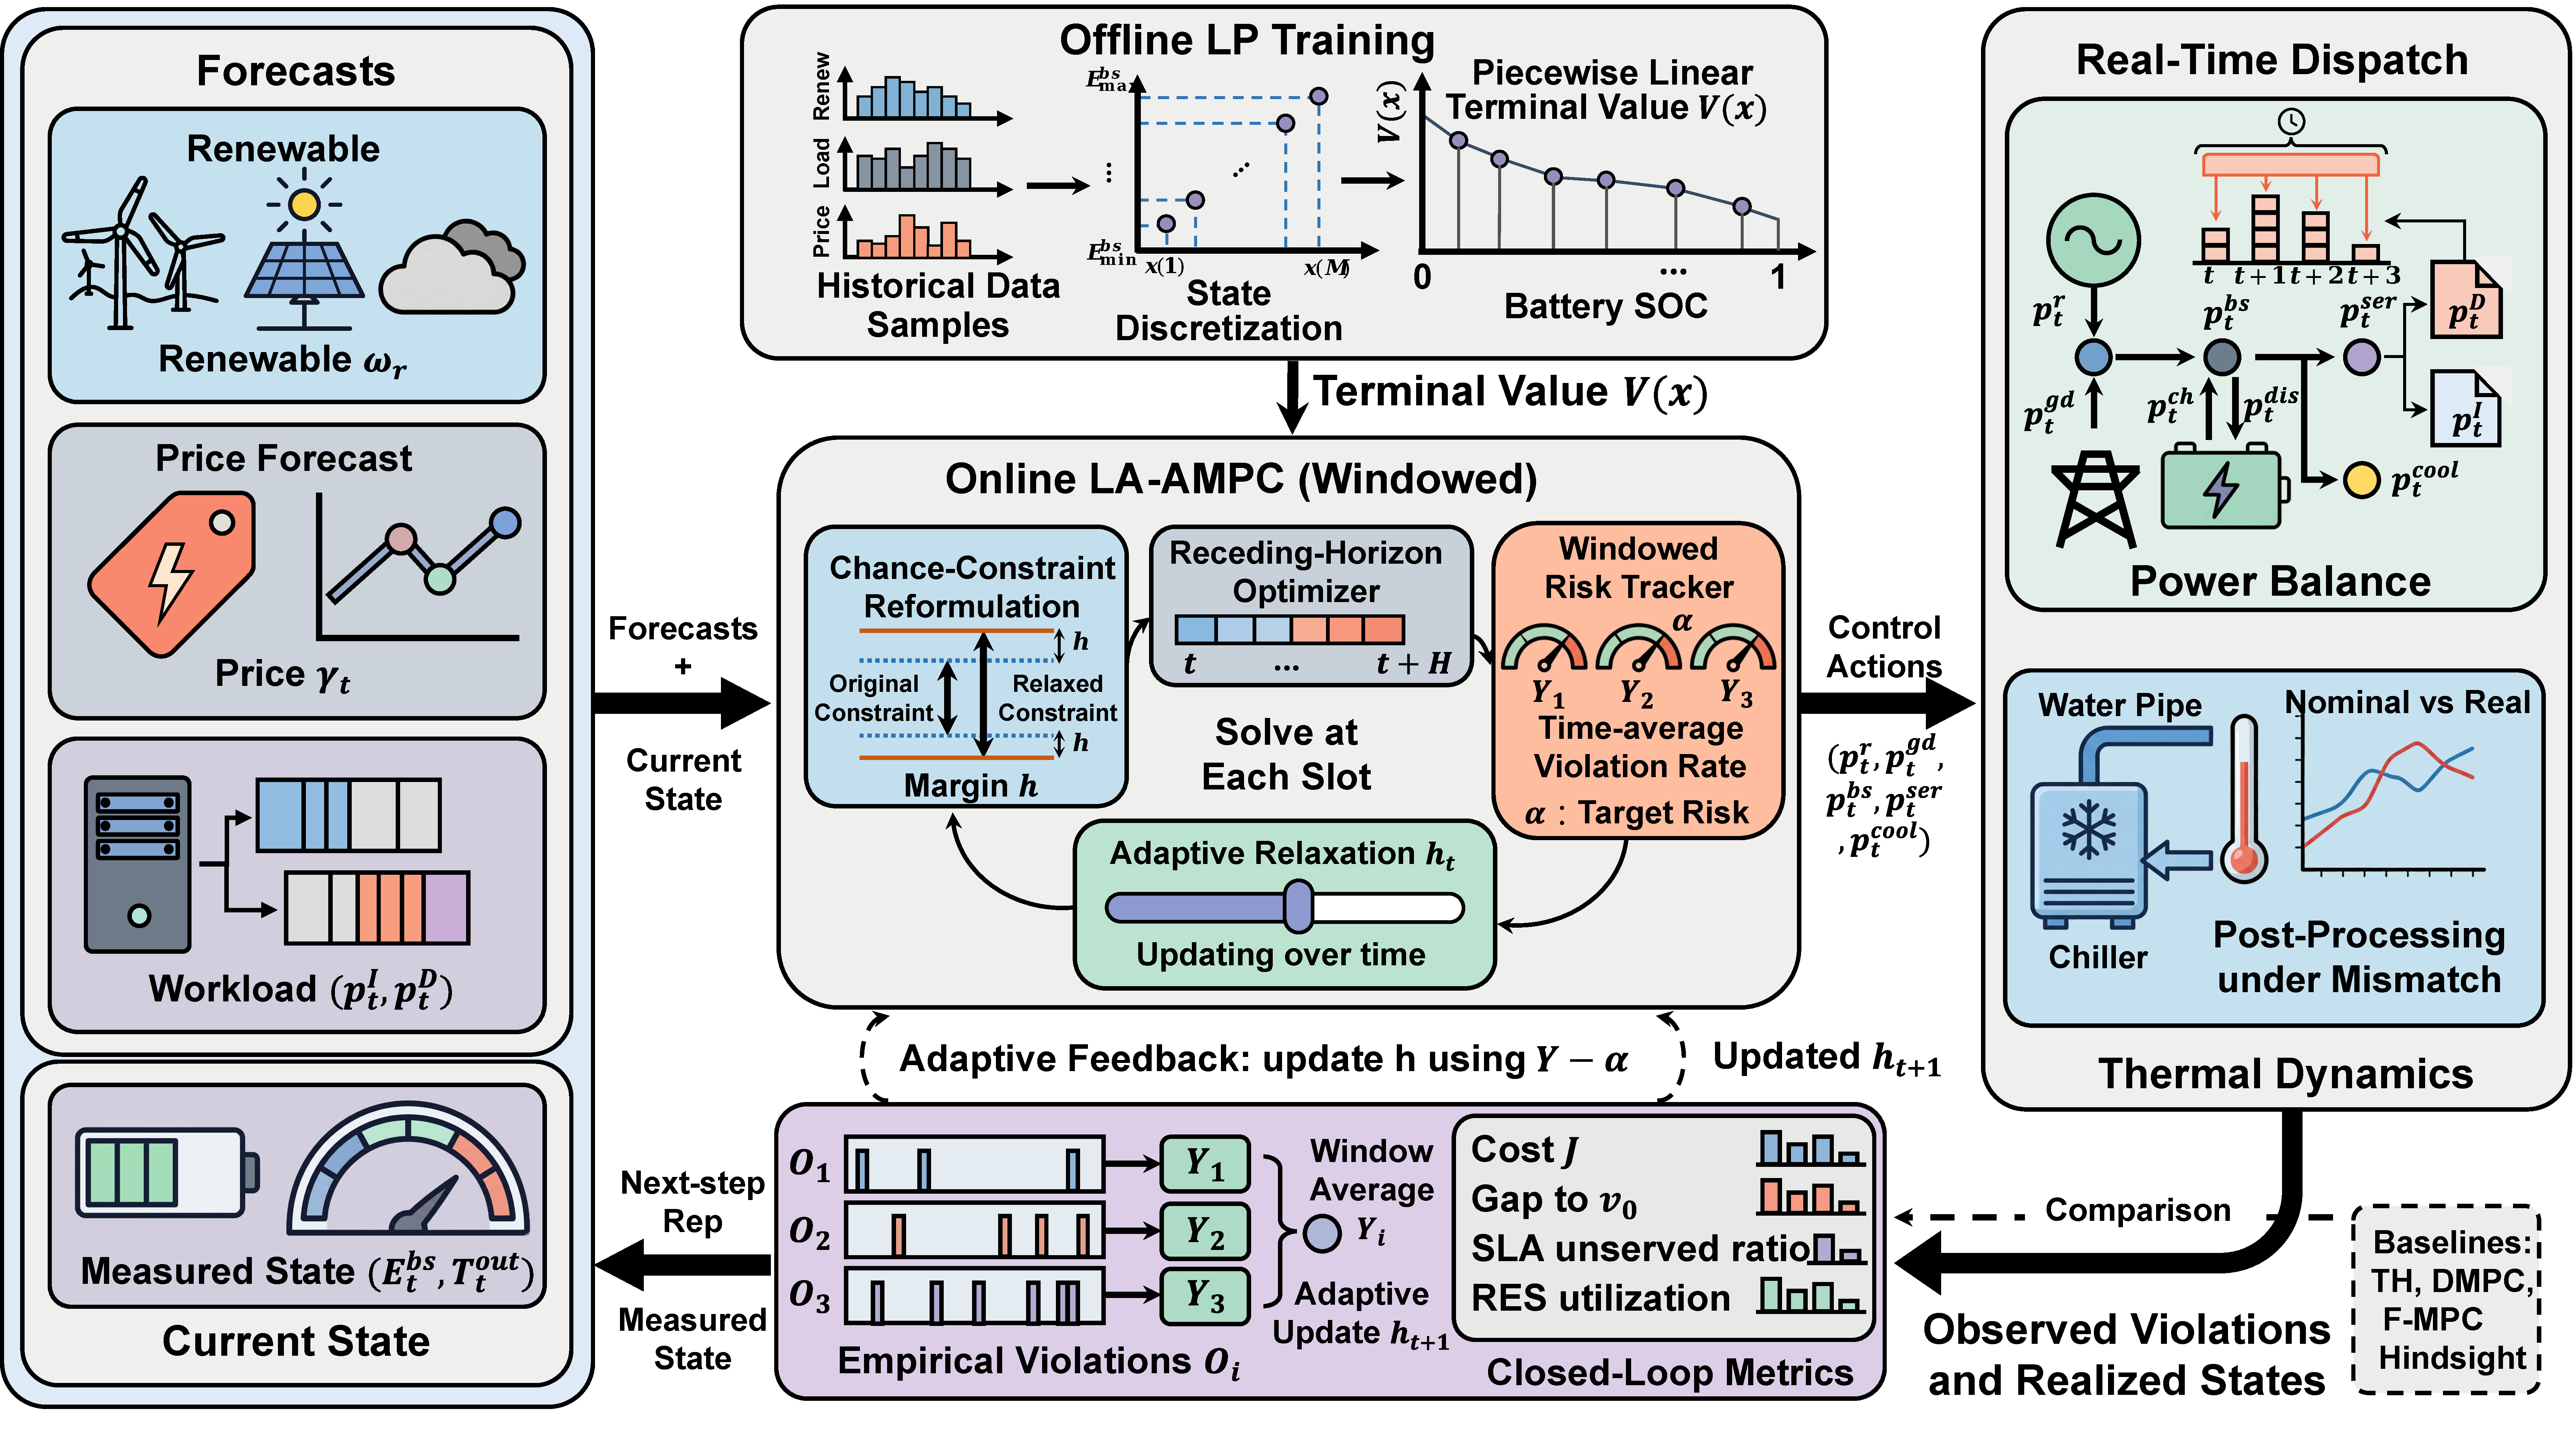
\includegraphics[width=0.95\textwidth,height=0.72\textheight,keepaspectratio]{fig_method_flow/method_flow_overview.pdf}
\caption{Overall workflow of the proposed learning-assist adaptive MPC framework.
From left to right, forecast inputs and measured states feed the online controller; offline LP training provides the terminal value approximation $V(x)$; the online module performs chance-constraint reformulation, receding-horizon optimization, and windowed risk tracking with adaptive relaxation updates; real-time dispatch and post-processing generate realized states and violation observations, which are fed back to update $h$.}
\label{fig:method_flow_overview}
\end{figure*}

\subsection{Chance Constraints Reformulation}
Following~\cite{ghosh2025_adaptive_relaxation_ccsmpc}, adaptive chance constraints are imposed on three state limits, namely the ESS lower bound, the ESS upper bound, and the outlet temperature upper bound. Throughout this paper, the pointwise-in-time chance constraints are reinterpreted as closed-loop time-average violation rate targets, since their strict probabilistic enforcement under unknown uncertainty distribution is generally over-conservative~\cite{ghosh2025_adaptive_relaxation_ccsmpc}. Let $H$ denote the MPC prediction horizon. Over this horizon, the pointwise chance constraints are
\begin{equation}\label{chance constraints 2}
\begin{aligned}
\mathbb{P}\!\left(E_{t+\ell}^{bs}\ge E_{\min}^{bs}\right) &\ge 1-\alpha_1,\\
\mathbb{P}\!\left(E_{t+\ell}^{bs}\le E_{\max}^{bs}\right) &\ge 1-\alpha_2,\\
\mathbb{P}\!\left(T_{t+\ell}^{out}\le T_{\max}^{out}\right) &\ge 1-\alpha_3,
\end{aligned}
\qquad \ell=1,\ldots,H.
\end{equation}
Here, $\alpha_1$, $\alpha_2$, and $\alpha_3$ are the target violation probabilities for the ESS lower bound, ESS upper bound, and thermal constraint, respectively.

To reduce closed-loop conservatism, adaptive relaxation variables $h_t^1$, $h_t^2$, and $h_t^3$ with $h_t^i\le 0$ are introduced, and the current relaxation values are applied uniformly to all predicted steps within the horizon. The restriction $h_t^i\le 0$ confines the adaptive bound to remain no tighter than the nominal limit; tightening toward the nominal value is achieved by driving $h_t^i$ back toward $0$, not by allowing $h_t^i>0$. The resulting MPC reformulation is
\begin{equation} \label{MPC chance con}
\begin{aligned}
E_{\min}^{bs}+h_t^1 &\le E_{t+\ell}^{bs},\\
E_{t+\ell}^{bs} &\le E_{\max}^{bs}-h_t^2,\\
T_{t+\ell}^{out} &\le T_{\max}^{out}-h_t^3,
\end{aligned}
\qquad \ell=1,\ldots,H,\ \forall t.
\end{equation}
Thus, at each decision epoch, one triplet $(h_t^1,h_t^2,h_t^3)$ is computed and enforced uniformly over the entire prediction horizon; its online update law is introduced next.

\subsection{Adaptive Adjustment}\label{subsec:adaptive_adjustment}
For compact notation, let $s_{t+1}:=[E_{t+1}^{bs},T_{t+1}^{out}]^\top$ denote the realized next-step state used to evaluate constraint violations. The three realized state limits in \eqref{chance constraints 2} can be written as $G_i s_{t+1}\le g_i$, $i=1,2,3$, with
$(G_1,g_1)=([-1,0],-E_{\min}^{bs})$, $(G_2,g_2)=([1,0],E_{\max}^{bs})$, and $(G_3,g_3)=([0,1],T_{\max}^{out})$,
corresponding to the ESS lower bound, ESS upper bound, and outlet temperature upper bound, respectively. Let $O^{i}_{t+1} \in \{0,1\}$ indicate whether the $i$-th realized limit is violated at time $t+1$, and let $Y^{i}_{t+1} \in [0,1]$ track its time-average violation rate up to time $t+1$:
\begin{equation}\label{eq:Oi_def}
O^i_{t+1} :=
\begin{cases}
1, & G_i s_{t+1} > g_i,\\[2mm]
0, & G_i s_{t+1} \le g_i,
\end{cases}
\end{equation}
\begin{equation*}
Y_{t+1}^i := \frac{\sum_{j=1}^{t+1} O^i_j}{t+1}.
\end{equation*}

Note that the control input applied at time $t$, together with the realized uncertainty at time $t$, affects the system state only at time $t+1$. This creates a one-step delay in observing whether a violation has occurred.

The original update rule of~\cite{ghosh2025_adaptive_relaxation_ccsmpc} applies a multiplicative correction $h_t^i = h_{t-1}^i\big[1+\big(\alpha_i - Y_t^i + (2Y_t^i-1)/(2(t+1))\big)/\chi_i\big]$ driven by the historical average $Y_t^i:=\sum_{j=1}^{t}O_j^i/t$, where $\chi_i$ is a proportionality constant controlling the update rate. Theorem~2 of~\cite{ghosh2025_adaptive_relaxation_ccsmpc} shows that, under ideal control inputs, $Y_t^i$ asymptotically converges to $\alpha_i$.

However, $Y_t^i$ measures the historical average violation rate from the initial time $t_0$ up to time $t$. As $t$ grows, the marginal contribution of each new observation $O_{t+1}^i$ to $Y_t^i$ decays as $1/(t+1)$, so $Y_t^i$ becomes increasingly insensitive to recent violations. Consequently, the historical average may remain close to $\alpha_i$ while the recent violation rate deviates from $\alpha_i$.

Since industrial practice often emphasizes recent controller performance, we restrict the computation of $Y_t^i$ to a predefined time window $w$. The recent average violation rate is then defined as
\begin{equation}\label{New Y}
    Y_t^{i,w} := \frac{\sum_{\tau = t-w+1}^{t}O_{\tau}^i}{w}, \quad \forall t\ge w,
\end{equation}
where $w$ is the window length. Correspondingly, the update rule for the adaptive relaxation parameter $h_t^{i,w}$ is modified as
\begin{equation}\label{update h new}
h^{i,w}_{t} = h^{i,w}_{t-1}\left[1+\frac{\alpha_i - Y_{t}^{i,w} + \frac{2O^{i}_{t-w+1}-1}{2w}}{\chi_i}\right], \quad \forall t\ge w.
\end{equation}
The numerator in~\eqref{update h new} gives the direction of the feedback. A positive numerator makes $h_t^{i,w}$ more negative, which relaxes the state limit and increases the chance of a violation at the next step. A negative numerator moves $h_t^{i,w}$ toward zero, which reduces the relaxation and lowers that chance.
The proportionality constant $\chi_i$ is chosen large enough that the multiplicative factor in~\eqref{update h new} remains positive for all $t$. Indeed, since $Y_t^{i,w}\in[0,1]$, $\alpha_i\in(0,1)$, and $O_{t-w+1}^i\in\{0,1\}$, the numerator $b_t^i:=\alpha_i-Y_t^{i,w}+(2O_{t-w+1}^i-1)/(2w)$ satisfies $|b_t^i|\le 1+1/(2w)$; thus any $\chi_i>1+1/(2w)$ guarantees $1+b_t^i/\chi_i>0$ and preserves $h_t^{i,w}<0$ once $h_{t_0}^{i,w}<0$.

Let $Z_t^{i,w} := \vert \alpha_i - Y_t^{i,w} \vert$ denote the absolute deviation between the target violation probability and the windowed empirical violation rate for the $i$-th state constraint at time $t$. The objective is to drive $Y_t^{i,w}$ toward $\alpha_i$ over time, i.e., to drive $Z_t^{i,w}$ to its minimum.

Let $\mathcal{F}_t = \left\{\xi_1, \xi_2, \dots, \xi_{t-1}\right\}$ represent the set of historical uncertainties up to time $t-1$. The quantity $Z_t^{i,w}$ is exactly known with information available up to time $t-1$, whereas $Z_{t+1}^{i,w}$ is random under $\mathcal{F}_t$. The following assumption and theorem summarize the convergence property of the windowed update law.

\begin{assumption}[Ideal one-step controllability]
For each constraint $i$ and time $t$, there exists an ideal policy that can determine the next-step violation event, namely $p_{t+1}^{i,*}\in\{0,1\}$ with $p_{t+1}^i:=P(O_{t+1}^i=1\mid \mathcal{F}_t)$.
\end{assumption}

\begin{theorem}[Convergence]\label{thm:window_conv}
Under Assumption~1, let $Y_t^{i,w,*}$ denote the windowed empirical violation rate generated by the ideal update law, and define $Z_t^{i,w,*}:=|\alpha_i-Y_t^{i,w,*}|$. Since $Y_t^{i,w,*}$ averages $w$ binary violation indicators, it can only take values on the grid $\{0,\tfrac{1}{w},\ldots,1\}$. The sequence $Z_t^{i,w,*}$ is monotonically nonincreasing and converges to $\min_{k=0,\ldots,w}|\alpha_i-k/w|$.
\end{theorem}

The formal statement and proof of Theorem~\ref{thm:window_conv} are given in Appendix~\ref{app:adaptive_mpc_proof}. Informally, under the ideal one-step controllability assumption, the windowed update law drives the empirical violation rate to the closest value achievable under the finite window length.

Under the ideal control policy $p_t^{i,w,*}$, the windowed empirical violation rate $Y_t^{i,w,*}$ eventually reaches the closest achievable value to $\alpha_i$. For sufficiently large window length $w$, the residual deviation from $\alpha_i$ becomes negligible. Hence, this result is the windowed counterpart of the historical-average convergence result in~\cite{ghosh2025_adaptive_relaxation_ccsmpc}.

\subsubsection*{Properties under a weaker attainability assumption}
Assumption~1 grants the controller a deterministic choice of the next-step violation event $O_{t+1}^i\in\{0,1\}$, which is a strong condition. In practice, the MPC solver only selects setpoints, and the resulting violation probability $p_{t+1}^i$ is determined jointly by the solver, dynamics, and forecast errors. To bridge this gap, we state a weaker attainability assumption and derive three complementary properties of the windowed update law that do not rely on the oracle.

\begin{assumption}[Attainable Bernoulli-rate interval]\label{asm:attain}
For each constraint $i$ and time $t$, the controller can select the conditional violation probability
$p_{t+1}^i := \mathbb{P}(O_{t+1}^i=1\mid \mathcal{F}_t)$ within an $\mathcal{F}_t$-measurable interval
$\mathcal{P}_t \supseteq [\underline p^i,\overline p^i]$, where $[\underline p^i,\overline p^i]\subseteq(0,1)$ is a deterministic conservative inner interval. Define the projected target
$\alpha_i^\star := \mathrm{proj}_{[\underline p^i,\overline p^i]}(\alpha_i)$.
\end{assumption}

Assumption~\ref{asm:attain} replaces the deterministic event-level choice in Assumption~1 by a probabilistic interval-level choice. When $[\underline p^i,\overline p^i]=[0,1]$ and the oracle is allowed to take the degenerate endpoints, Assumption~1 is recovered.

\begin{proposition}[One-step optimality]\label{prop:onestep}
Under Assumption~\ref{asm:attain}, the windowed update rule \eqref{update h new}, interpreted as the extreme-point selection rule that selects $\overline p^i$ when $\varphi_t^\star<0$ and $\underline p^i$ when $\varphi_t^\star>0$ (with $\varphi_t^\star$ defined in Appendix~\ref{app:adaptive_mpc_proof}, Section~\ref{subsec:weak}), minimizes the one-step conditional expected absolute tracking error $\mathbb{E}\!\left[|Y_{t+1}^{i,w}-\alpha_i^\star|\,\middle|\,\mathcal{F}_t\right]$ over $p_{t+1}^i\in[\underline p^i,\overline p^i]$.
\end{proposition}

\begin{proposition}[Structural lower bound]\label{prop:lower}
Under Assumption~\ref{asm:attain}, for any control policy with $p_t^i\in[\underline p^i,\overline p^i]$ admitting a stationary distribution $\rho^\star$,
\begin{equation}\label{eq:lower-bound}
\mathbb{E}_{\rho^\star}|Y_t^{i,w}-\alpha_i|\,\ge\,|\alpha_i-\alpha_i^\star|.
\end{equation}
\end{proposition}

\begin{proposition}[Constructive upper bound]\label{prop:upper}
The constant policy $p_t^i\equiv\alpha_i^\star$ is feasible under Assumption~\ref{asm:attain} and achieves
\begin{equation}\label{eq:upper-bound}
\mathbb{E}\,|Y_t^{i,w}-\alpha_i|\,\le\,|\alpha_i-\alpha_i^\star|+\tfrac{1}{2\sqrt{w}},
\end{equation}
with concentration $\mathbb{P}\!\left[|Y_t^{i,w}-\alpha_i^\star|>\epsilon\right]\le 2\exp(-2w\epsilon^2)$ for any $\epsilon>0$.
\end{proposition}

Propositions~\ref{prop:onestep}--\ref{prop:upper} jointly characterize the attainable performance of the windowed mechanism without the oracle. Their formal statements and proofs are given in Appendix~\ref{app:adaptive_mpc_proof}. The combination $|\alpha_i-\alpha_i^\star|+\mathcal{O}(1/\sqrt{w})$ provides a structural performance envelope: the unattainability gap $|\alpha_i-\alpha_i^\star|$ cannot be eliminated by any policy in $[\underline p^i,\overline p^i]$, but is achievable up to a $\mathcal{O}(1/\sqrt{w})$ residual.

\begin{remark}\label{rem:gap}
The W-policy abstraction provides a tractable theoretical reference under the ideal one-step controllability assumption. The actual $h$-update implemented in Algorithm~\ref{alg:oa_smpc_pp_concise} affects $p_{t+1}^i$ only indirectly through the MPC solver, and its closed-loop behavior may differ from (and, as shown empirically in Section~\ref{sec:case_studies}, exceed) the W-policy idealization. We report empirical convergence to $\alpha_i$ as the primary validation; the W-policy analysis serves as a qualitative consistency check rather than a tight theoretical bound.
\end{remark}

\begin{remark}[Sense of chance-constraint satisfaction]\label{rem:cc-sense}
Closed-loop risk tracking is assessed by how closely the windowed empirical violation rate $Y_t^{i,w}$ follows the target $\alpha_i$. This criterion does not imply strict pointwise probabilistic satisfaction of~\eqref{chance constraints 2}.
\end{remark}


\subsection{Online Adaptive MPC}
The online MPC decision vector is
\[\boldsymbol{x}_t^e = \{p_t^r,\, p_t^{gd},\, p_t^{\text{ch}},\, p_t^{\text{dis}},\, p_t^{bs},\, E_t^{bs},\, T_t^{chw},\, c_{\tau,k,t}^D\}.\]
Let $t_0$ denote the current decision epoch and $\mathcal{A}_{t_0}$ the active deferrable-demand set at epoch $t_0$, including unfinished past arrival groups and predicted arrivals within the MPC horizon.
For each $(\tau,k)\in\mathcal{A}_{t_0}$, define the remaining CPU-time demand $\hat{C}_{\tau,k}^D(t_0)$, the absolute deadline $d_{\tau,k}:=\min(\tau+D_k,\ T)$, and the receding-horizon execution window
$\mathcal{W}_{\tau,k}^{(t_0)} := \{\max(\tau,t_0),\max(\tau,t_0)+1,\ldots,\min(d_{\tau,k},\,t_0+H)\}$.
The terminal remaining demand is then
$\hat{C}_{\tau,k}^D(t_0{+}H):=\hat{C}_{\tau,k}^D(t_0)-\sum_{t\in \mathcal{W}_{\tau,k}^{(t_0)}} c_{\tau,k,t}^D \Delta\tau$.
Throughout this section, the hat denotes a measured or known quantity at the current decision epoch, such as the remaining demand $\hat{C}_{\tau,k}^D(t_0)$ and the measured state components $\hat{E}_{t_0}^{bs}$ and $\hat{T}_{t_0}^{out}$.
We further split $\mathcal{A}_{t_0}$ into $\mathcal{A}_{t_0}^{\mathrm{in}}:=\{(\tau,k)\in\mathcal{A}_{t_0}\mid d_{\tau,k}\le t_0+H\}$ and $\mathcal{A}_{t_0}^{\mathrm{out}}:=\mathcal{A}_{t_0}\setminus\mathcal{A}_{t_0}^{\mathrm{in}}$, corresponding to deadlines inside and beyond the horizon, respectively.
At each decision epoch, the current state and current exogenous inputs are measured, whereas all exogenous quantities over the future prediction horizon are provided by short-term forecasts.

Collecting constraints \eqref{eq:pd}--\eqref{eq:pgd}, the resulting online adaptive MPC problem is formulated as follows:
\begin{subequations}\label{eq:total_problem}
\begin{align}
    \min\ & \gamma_{t_0}p_{t_0}^{gd}\Delta \tau + \sum_{t=t_0+1}^{t_0+H}\gamma_t p_t^{gd} \Delta \tau
           + V\left(E_{t_0+H}^{bs}\right) 
           \label{eq:total_problem_obj} \\
    \text{s.t. }\ &
    0 \leq p_{t}^r \leq \omega_{t}^r ,\forall t  \\
    &
    p_t^r + p_t^{gd}
    = p_t^{bs} + p_t^{\text{ser}} + p_t^{\text{cool}},
    \forall t
    \label{eq:total_problem_balance} \\
    &
    E_{\min}^{bs} + h_t^1 \leq E_t^{bs}
    \leq E_{\max}^{bs} - h_t^2,
    \forall t
    \label{eq:total_problem_E_bounds} \\
    &
    T_t^{out} \leq T_{\max}^{out} - h_t^3,
    \forall t
    \label{eq:total_problem_T_out_bound} \\
    & E_{t_0}^{bs} = \hat{E}_{t_0}^{bs}, T_{t_0}^{out} = \hat{T}_{t_0}^{out} \label{eq:total_problem_init} \\
    &
    h_t^i \le 0,
    \forall i\in\{1,2,3\},\text{and } \forall t
    \label{eq:total_problem_h} \\
    & \sum_{t\in \mathcal{W}_{\tau,k}^{(t_0)}} c_{\tau,k,t}^D \,\Delta \tau
    = \hat{C}_{\tau,k}^D(t_0),
     \forall (\tau,k)\in\mathcal{A}_{t_0}^{\mathrm{in}}
    \label{eq:total_problem_sumC}\\
    & \begin{aligned}[t]
    0 \le \hat{C}_{\tau,k}^D(t_0{+}H) \le& M_k^D\!\left(d_{\tau,k}-t_0-H\right)\Delta\tau,\\
      & \forall (\tau,k)\in\mathcal{A}_{t_0}^{\mathrm{out}}
    \end{aligned}\\
    & 0 \le c_{\tau,k,t}^D \le M_k^D,
    \quad \forall (\tau,k)\in\mathcal{A}_{t_0},\ \forall t\in \mathcal{W}_{\tau,k}^{(t_0)}\\
    & c_t^{D} = \sum_{\tau=1}^{t}\sum_{k\in\mathcal{K}} c_{\tau,k,t}^D,\quad \forall t=t_0,\ldots,t_0+H
    \label{eq:total_problem_agg}\\
    & \boldsymbol{x}_t^e \text{ satisfies } \eqref{eq:pser},\ \eqref{eq:util},\ \eqref{eq:Cooling},\ \eqref{eq:Tchw},\ \eqref{eq:pgd},\ \eqref{eq:Ebs} 
\end{align}
\end{subequations}

The objective function \eqref{eq:total_problem_obj} consists of three components. The first term $\gamma_{t_0}p_{t_0}^{gd}\Delta \tau$ is the realized grid-purchase cost at the current slot $t_0$. The second term $\sum_{t=t_0+1}^{t_0+H}\gamma_t p_t^{gd} \Delta \tau$ is the forecast-based grid-purchase cost over the remaining horizon. The third term is the offline-trained terminal value $V(E_t^{bs})$, which is a monotonically decreasing, piecewise-linear, convex approximation of the beyond-horizon cost-to-go. Constraint~\eqref{eq:total_problem_balance} enforces power balance, constraints~\eqref{eq:total_problem_E_bounds} and \eqref{eq:total_problem_T_out_bound} are the relaxed reformulation of the chance constraints, and constraint~\eqref{eq:total_problem_h} restricts the relaxation variables to enlarge the feasible region only in the admissible direction. The state-initialization constraint \eqref{eq:total_problem_init} assigns the initial values of $E_{t_0}^{bs}$ and $T_{t_0}^{out}$ to the measured quantities $\hat{E}_{t_0}^{bs}$ and $\hat{T}_{t_0}^{out}$.

The workload constraints from \eqref{eq:total_problem_sumC} to \eqref{eq:total_problem_agg} enforce SLA feasibility and aggregation consistency at the arrival group level. Arrival groups whose deadlines fall inside the current MPC horizon must be fully completed, whereas those whose deadlines lie beyond the horizon are allowed to retain a terminal backlog only if it can still be cleared by the remaining service capacity after $t_0+H$. The per-slot bounds limit each group allocation by $M_k^D$, and \eqref{eq:total_problem_agg} aggregates the allocations $c_{\tau,k,t}^D$ into the slot-level deferrable decision $c_t^D$.


\subsection{Real-Time Implementation Under Cooling-Model Mismatch}\label{subsec:rt_impl}

The MPC in~\eqref{eq:total_problem} uses a simulation-calibrated cooling surrogate, so the metered cooling power may differ from the value embedded in~\eqref{eq:total_problem_balance}. At each epoch $t_0$, the first-step workload, chilled water setpoint, and storage commands are deployed, and the supply-side pair $(p_{t_0}^r,p_{t_0}^{gd})$ is then corrected after $\hat p_{t_0}^{cool}$ is measured. With $D_{t_0}^{\mathrm{act}}:=p_{t_0}^{bs,*}+p_{t_0}^{\text{ser}}+\hat{p}_{t_0}^{cool}$, this renewables-first correction is well defined when $0\le D_{t_0}^{\mathrm{act}}\le \omega_{t_0}^r+P_{\max}^{gd}$; under this condition it maximizes renewable use and assigns the residual demand to grid import. The complete logic is summarized in Algorithm~\ref{alg:oa_smpc_pp_concise}.

No separate post-processing is applied to $T_t^{out}$. Thermal-state mismatch is handled through receding-horizon feedback from the measured state $s_{t_0}=\{E_{t_0}^{bs},T_{t_0}^{out}\}$ and through the adaptive relaxation margin $h_t^3$, whose update reflects persistent thermal-model bias in the empirical violation statistics.

\begin{algorithm}[t]
\caption{Learning-assist adaptive MPC with renewables-first correction.}
\label{alg:oa_smpc_pp_concise}
\begin{algorithmic}[1]
\REQUIRE Terminal value function $V(\cdot)$ (offline); risk targets $\alpha_i$, gains $\chi_i$, window $w$; short-term forecasts over the next $H$ steps.
\REQUIRE At time $t$: measured $s_t=\{\hat{E}_t^{bs},\hat{T}_t^{out}\}$, realized $\xi_t$, active-set data $(\mathcal{A}_t,\hat{C}_{\tau,k}^D(t))$, metered $\hat{p}_t^{cool}$.
\ENSURE Implemented $T_t^{chw}$, $\{c_{\tau,k,t}^D\}$, $(p_t^r,p_t^{gd})$, $(p_t^{ch},p_t^{dis})$; updated $h_{t+1}$.

\STATE Initialize $h_0\le 0$ and violation-history buffer; set $t\leftarrow 0$.
\WHILE{$t\le T-1$}
    \STATE Solve \eqref{eq:total_problem} with the measured current inputs, the short-term forecasts over the next $H$ steps, and $h_t$ to obtain the first-step setpoints $x_{t}^{e,*}$.
    \STATE Deploy nominal commands: $T_t^{chw}\!\leftarrow\!T_t^{chw,*}$, $c_{\tau,k,t}^D\!\leftarrow\!c_{\tau,k,t}^{D,*}$, $(p_t^{ch},p_t^{dis})\!\leftarrow\!(p_t^{ch,*},p_t^{dis,*})$.
    \STATE Compute the power-balance residual
    $r_t := \big(p_t^{bs,*}+p_t^{\text{ser}}+\hat{p}_t^{\text{cool}}\big)-\big(p_t^{r,*}+p_t^{gd,*}\big)$.
    \IF{$r_t>0$}
        \STATE $p_t^r \leftarrow \min\{\omega_t^r,\ p_t^{r,*}+r_t\}$; \quad
               $p_t^{gd} \leftarrow \min\{P_{\max}^{gd},\ p_t^{gd,*}+r_t-(p_t^r-p_t^{r,*})\}$.
    \ELSE
        \STATE $p_t^{gd} \leftarrow \max\{0,\ p_t^{gd,*}+r_t\}$; \quad
               $p_t^{r} \leftarrow \max\{0,\ p_t^{r,*}+r_t-(p_t^{gd}-p_t^{gd,*})\}$.
    \ENDIF
    \STATE Observe $s_{t+1}$ and, for all $i\in\{1,2,3\}$, compute $O_{t+1}^i$ by \eqref{eq:Oi_def}, update $Y_{t+1}^{i,w}$ by \eqref{New Y}, and update $h_{t+1}^{i,w}$ by \eqref{update h new}.
    \STATE Set $h_{t+1}\leftarrow (h_{t+1}^{1,w},h_{t+1}^{2,w},h_{t+1}^{3,w})$ and $t\leftarrow t+1$.
\ENDWHILE
\end{algorithmic}
\end{algorithm}



\section{Case Studies}\label{sec:case_studies}
\subsection{Experimental Setup}
We consider a single data center equipped with on-site renewable generation, a battery ESS,
and a grid connection. The system is operated in 15-min time slots, and the online controller is executed in a
receding-horizon manner. Key system limits and controller settings are summarized in Table~\ref{tab:exp_params}.

\begin{table}[!htbp]
\caption{Key parameters used in the case studies.}
\label{tab:exp_params}
\centering
\footnotesize
\setlength{\tabcolsep}{4pt}
\renewcommand{\arraystretch}{1.05}
\begin{tabularx}{\linewidth}{@{}Xcr@{}}
\toprule
Parameter & Symbol & Value \\
\midrule
Time slot length & $\Delta\tau$ & 15 min \\
Slots per day & $|\mathcal{T}|$ & 96 \\
MPC horizon & $H$ & 4 slots (1 h) \\
Grid import limit & $P_{\max}^{gd}$ & 15 MW \\
PV/Wind rated capacity & $(P_{\max}^{pv},P_{\max}^{w})$ & (10, 20) MW \\
ESS power limit & $P_{\max}^{bs}$ & 5 MW \\
ESS energy bounds & $[E_{\min}^{bs},E_{\max}^{bs}]$ & [5, 20] MWh \\
ESS efficiencies & $(\eta_{\mathrm{ch}},\eta_{\mathrm{dis}})$ & (0.97, 0.98) \\
Chilled water supply setpoint bounds & $[T_{\min}^{chw},T_{\max}^{chw}]$ & [15, 24] $^\circ$C \\
Setpoint ramp limit & $\zeta$ & 2 $^\circ$C/h \\
Server outlet air temperature limit & $T_{\max}^{out}$ & 26 $^\circ$C \\
Risk targets (ESS low/high, temp) & $\boldsymbol{\alpha}$ & (0.1, 0.1, 0.1) \\
Sliding-window length & $w$ & 2880 slots (30 days) \\
Adaptation gains & $\boldsymbol{\chi}$ & (10, 10, 15) \\
Deferrable SLA classes & $K$ & 3 \\
Deadlines (in slots) & $D_k$ & (3, 4, 5) \\
Per-slot deferrable cap & $M_k^D$ & (5, 5, 5) \\
\bottomrule
\end{tabularx}
\end{table}

\noindent\textbf{Data sources.}
Workload traces are derived from the Google Open Trace (cluster trace) dataset~\cite{google2019_cluster_trace}, and real-time electricity
prices are from the PJM market~\cite{pjm_dataminer2}. Renewable generation and ambient-condition traces are aligned to the same 15-min resolution.
% Reproducibility details pending author records: Google trace version, selected cells,
% dates/fields, workload-class mapping, scaling, 15-min aggregation, and construction
% of the multi-year sequence; PJM feed, node/region, dates/time zone, price field/unit,
% aggregation, and handling of negative prices and missing observations.

\noindent\textbf{Uncertainty and forecasting.}
At each slot $t$, the controller observes the realized uncertainty $\xi_t$ and uses short-term forecasts of renewable generation, electricity price, and workload arrivals over the next $H$ slots.
In the main closed-loop experiments, these forecasts are produced by direct multi-step long short-term memory (LSTM) models trained from the historical traces at the 15-min resolution. Each predictor uses the latest one-day history and calendar features to generate the next $H=4$ forecasts, and the prediction is updated after each newly observed slot.

The forecasting module was evaluated by a 31-day rolling-origin test using the realized history available at each prediction time. The normalized mean absolute errors are $7.97\%$ for renewable generation, $4.37\%$ for deferrable workload, and $5.20\%$ for interactive workload, with forecast bias below $1.4\%$ of the corresponding mean realized value. The electricity-price forecast has an MAE of $4.96$ USD/MWh and a small MBE of $-0.36$ USD/MWh. Thus, the closed-loop experiments use data-driven forecast residuals rather than manually prescribed multiplicative disturbances, and the forecast-error robustness sweep scales the empirical LSTM residuals.

\noindent\textbf{Controller implementation.}
The online MPC is modeled in YALMIP and solved as a linear program by Gurobi Optimizer 11.0.3 on a Windows 11 machine with an Intel Core i7-14700HX CPU and 32\,GB RAM. At each step, the controller follows the closed-loop sequence: measure $\rightarrow$ optimize $\rightarrow$ implement the first-step actions $\rightarrow$ update.

\noindent\textbf{Fairness of comparison.}
All compared methods use the same dataset, exogenous trajectories, point forecasts, and solver configuration. The same system parameters and physical limits are enforced across methods; the methods differ only in their control-policy design.
\subsection{Compared Methods and Metrics}
\noindent\textbf{Compared methods.}
We benchmark the proposed LA-AMPC against the following baselines.
Unless otherwise stated, all controllers share the same system model and constraints, use the same measurements at the
current slot, and rely on the same point forecasts over the next $H$ steps.

\noindent\textbf{(0) Hindsight (ex-post) optimum ($v_0$).}
A non-causal ex-post baseline is defined by solving a full-day deterministic problem with perfect knowledge of renewables, prices, and workloads; since this benchmark uses future information, it is not implementable online, and the resulting daily cost $v_0$ is used only as the reference for the reported optimality gap.

\noindent\textbf{(1) Threshold policy (TH).}
Deferrable workloads are scheduled by an earliest-deadline-first (EDF) rule across the $K$ SLA classes, subject to the per-slot caps $M_k^D$ and the IT capacity.
Cooling is controlled by a temperature threshold $\bar{T}$: if $T_t^{out}>\bar{T}$, the chilled water supply setpoint is decreased by the maximum allowable ramp, i.e., $T_t^{chw}\leftarrow\max\{T_{\min}^{chw},\,T_{t-1}^{chw}-\zeta\Delta\tau\}$; otherwise $T_t^{chw}=T_{t-1}^{chw}$.
The ESS uses two energy thresholds $\underline{E}$ and $\overline{E}$: it charges if $E_t^{bs}<\underline{E}$, discharges if $E_t^{bs}>\overline{E}$, and otherwise charges using any renewable surplus, all subject to power and energy limits.
All thresholds are tuned offline by Bayesian optimization on a validation set.

\noindent\textbf{(2) Deterministic/nominal MPC (DMPC).}
DMPC uses the same receding-horizon optimization model, point forecasts, and terminal-value term as LA-AMPC, but fixes the adaptive relaxation vector to zero, i.e., $h_t\equiv 0$, so that the ESS and thermal states are constrained by the nominal deterministic bounds without any online relaxation update.

\noindent\textbf{(3) Fixed-relaxation MPC (F-MPC)~\cite{ghosh2025_adaptive_relaxation_ccsmpc}.}
Following the ``Traditional EMPC2'' benchmark in~\cite{ghosh2025_adaptive_relaxation_ccsmpc}, this baseline uses the same initial relaxation as LA-AMPC but keeps it fixed in closed loop, thereby isolating the contribution of the online adaptive relaxation.

\noindent\textbf{Metrics.}
We report: (i) operating cost $J:=\sum_{t}\gamma_t p_t^{gd}\Delta\tau$; (ii) optimality gap to the hindsight benchmark
$v_0$, $\mathrm{Gap}:=(J-v_0)/v_0$; (iii) time-average empirical violation rates $Y_t^{i,w}$; (iv) SLA performance via the unserved CPU-time ratio
$\rho_{\mathrm{SLA}}:=\frac{\sum_{\tau,k}(C_{\tau,k}^D-\sum_{t\in\mathcal{W}_{\tau,k}}c_{\tau,k,t}^D\Delta\tau)_+}{\sum_{\tau,k}C_{\tau,k}^D}$;
(v) renewable-utilization ratio $\eta_{\mathrm{RES}}:=\frac{\sum_t p_t^r}{\sum_t \omega_t^r}$ (equivalently, curtailment).

\subsection{Offline Training and Convergence Behavior}
Fig.~\ref{fig:offline_value} can be read as a boundary-triggered price-threshold map induced by the terminal value function.
The learned profile is nonincreasing: a higher storage level corresponds to a smaller terminal value, consistent with the role of stored energy in reducing future grid purchases.
The nominal ESS-energy band is $[5,20]$ MWh, whereas the physical band is $[0,25]$ MWh.
Crossing the nominal boundary is therefore economically meaningful only under sufficiently strong price signals.
At the lower bound, discharging from $5$ MWh below $5$ MWh is preferred only when the instantaneous energy-price benefit exceeds the marginal terminal-value loss, i.e., approximately $\gamma_t\Delta\tau > -\Delta V/\Delta x$ around $x=5$ (with efficiency correction in implementation).
At the upper bound, charging above $20$ MWh is preferred only when the price is low enough that the charging gain dominates the marginal decrease of $V(x)$ around $x=20$.
Boundary violations are therefore conditional and are activated only when the immediate arbitrage value dominates the terminal-value penalty.

\begin{figure}[!htbp]
\centering
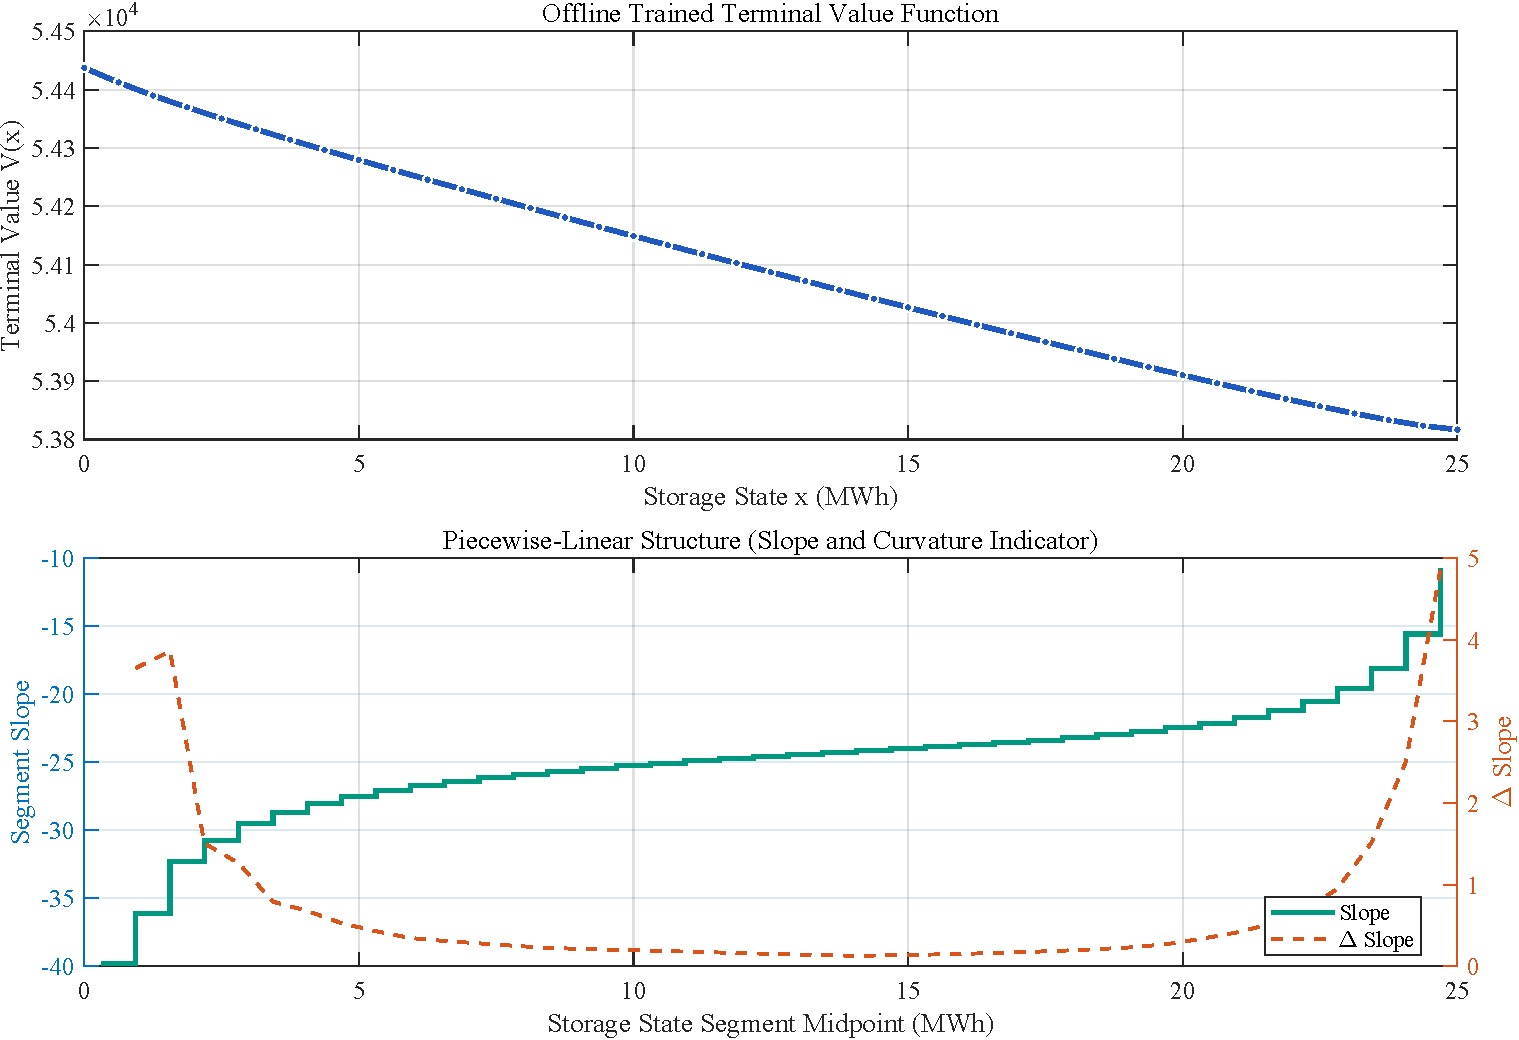
\includegraphics[width=\columnwidth,height=0.72\textheight,keepaspectratio]{fig_offline_training/fig1_offline_value_function.pdf}
\caption{Offline-trained terminal value function $V(x)$ and its piecewise-linear slope profile.}
\label{fig:offline_value}
\end{figure}

Fig.~\ref{fig:Y_convergence_window} jointly shows the empirical violation statistic $Y_i$ and the paired adaptive relaxation variable $h_i$. The moving averages of $Y_1$, $Y_2$, and $Y_3$ remain around the target level $\alpha$, while $h_i$ moves in the opposite direction as the risk pressure changes. The daily curves still exhibit visible oscillations, so the convergence in real-world complex systems should be interpreted as stable tracking in an average sense, rather than strict monotonic convergence on each day.

\begin{figure}[!htbp]
\centering
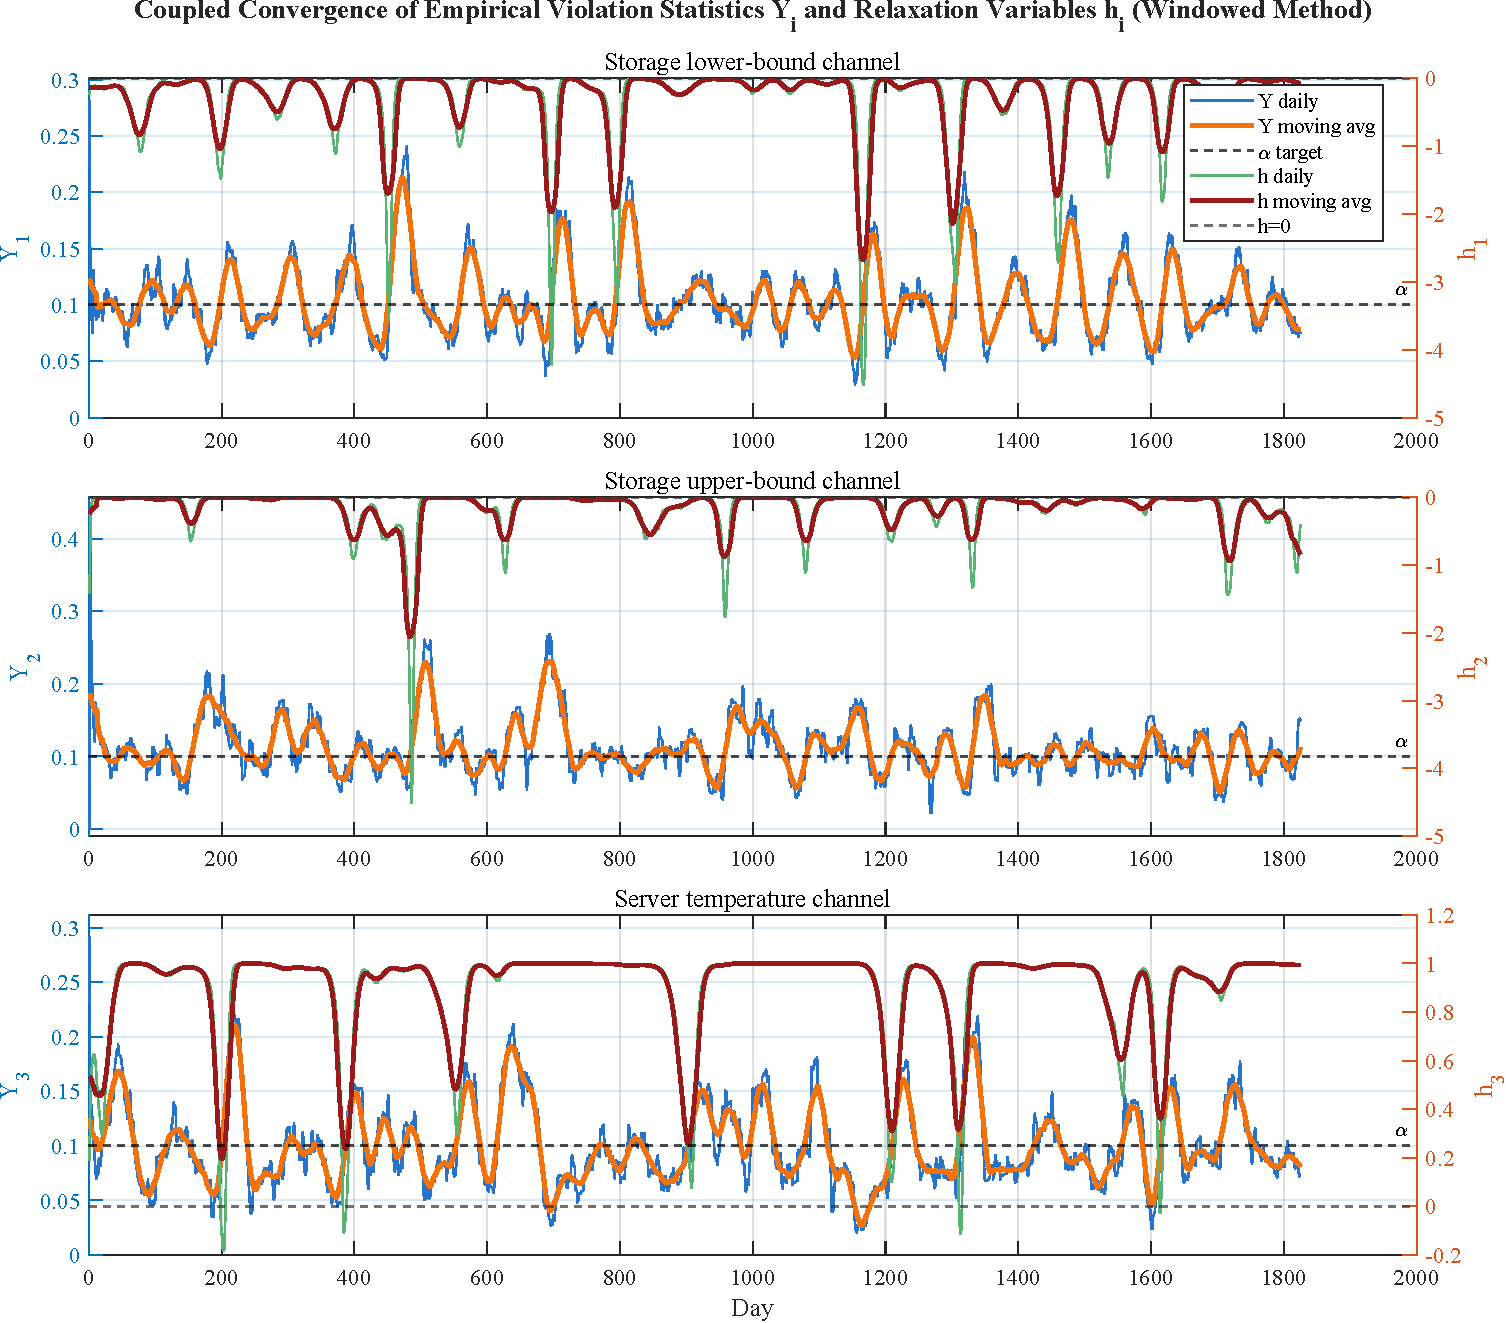
\includegraphics[width=\columnwidth,height=0.72\textheight,keepaspectratio]{fig_offline_training/fig3_Yh_convergence_window.pdf}
\caption{Combined convergence view for the windowed method: left axis shows $Y_1,Y_2,Y_3$ (daily and moving-average),
right axis shows the paired adaptive relaxation variables $h_1,h_2,h_3$.}
\label{fig:Y_convergence_window}
\end{figure}
\subsection{Main Closed-Loop Performance}
The closed-loop trajectories of the windowed controller are first examined on a representative operating day. These trajectory plots are used to illustrate the qualitative closed-loop mechanisms, while aggregate performance is reported separately in Table~\ref{tab:main_closedloop_compare} and Fig.~\ref{fig:main_daily_distribution}.

Fig.~\ref{fig:main_typical_dispatch} reports supply-side dispatch and workload execution on this operating day. The controller uses available renewables before grid imports, and the cumulative processed demand $D(t)$ remains between $A(t)$ and $D_{\min}(t)$, indicating compliance with the aggregate workload-balance and cumulative service bounds. Individual arrival-group deadline constraints are imposed by~\eqref{eq:pd}. During high-renewable periods, $D(t)$ approaches $A(t)$, showing proactive service of backlog and newly arrived workload groups to improve renewable utilization.

\begin{figure}[!htbp]
\centering
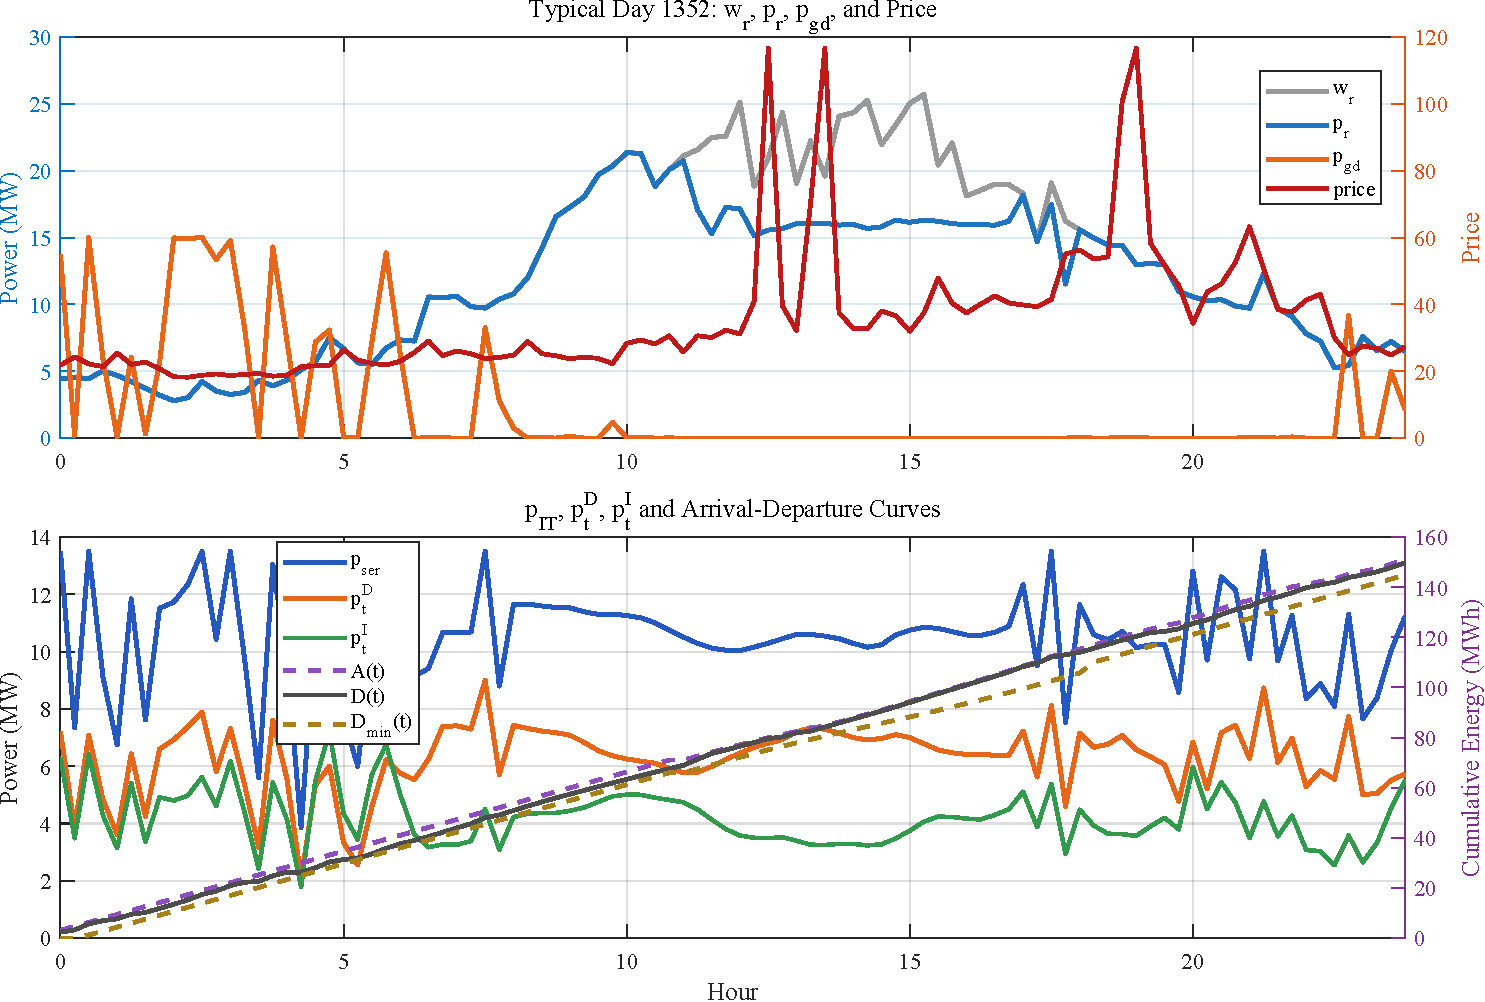
\includegraphics[width=\columnwidth,height=0.72\textheight,keepaspectratio]{fig_main_closedloop/fig_main_typical_day_dispatch.pdf}
\caption{Typical-day dispatch behavior of the proposed windowed controller. Top: $\omega_t^r$, $p_t^r$, $p_t^{gd}$, and price.
Bottom: $p_t^{ser}$, $p_t^D$, $p_t^I$, and cumulative arrival--departure curves
($A(t), D(t), D_{\min}(t)$).}
\label{fig:main_typical_dispatch}
\end{figure}

Fig.~\ref{fig:main_typical_states} shows the storage and thermal trajectories with their associated control actions. The ESS temporarily exceeds the nominal upper bound during high-renewable periods to absorb additional energy, and persistent violations are followed by an increase in $h$ that tightens the effective constraint and drives the state back toward the nominal range.

The lower panel separates nominal planning and realized execution under thermal-model mismatch: $T_t^{out,\mathrm{nom}}$ and $p_t^{cool,\mathrm{nom}}$ are generated by the optimization model, whereas $T_t^{out,\mathrm{real}}$ and $p_t^{cool,\mathrm{adj}}$ are the realized and post-processed trajectories. Their gap confirms that model mismatch is non-negligible and that the real-time correction layer is needed to preserve power-balance feasibility.


\begin{figure}[!htbp]
\centering
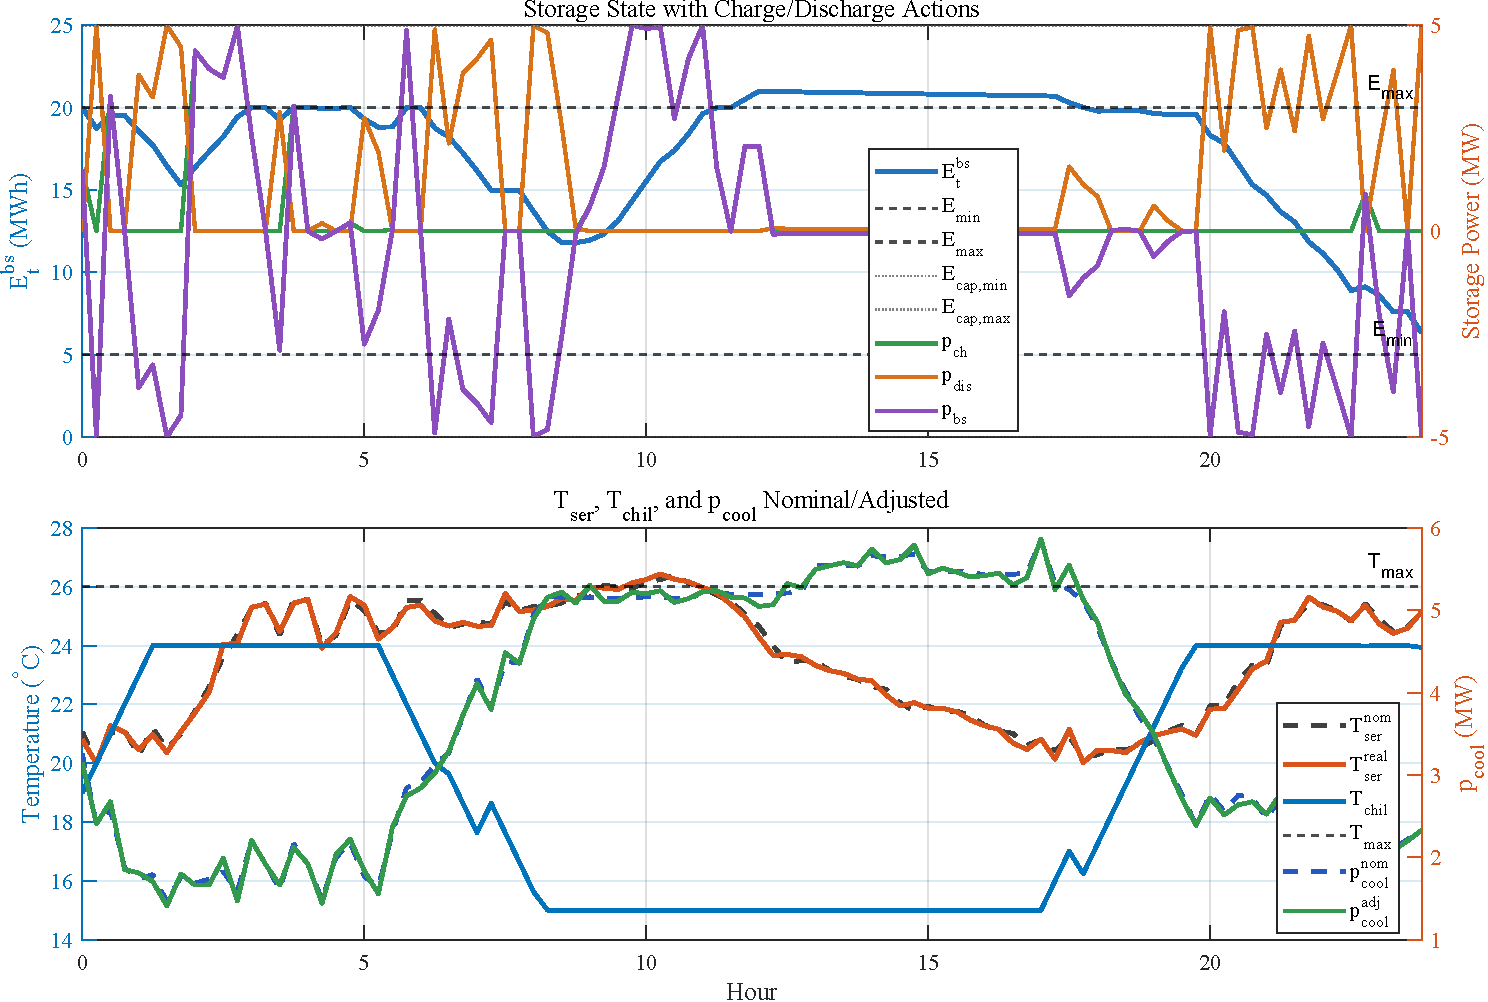
\includegraphics[width=\columnwidth,height=0.72\textheight,keepaspectratio]{fig_main_closedloop/fig_main_typical_day_states.pdf}
\caption{Typical-day storage and thermal behavior of the proposed windowed controller. Top: storage state $E_t^{bs}$ with
nominal/physical bounds and storage powers ($p_t^{ch}, p_t^{dis}, p_t^{bs}$). Bottom: $T_t^{out,nom}$ vs. $T_t^{out,real}$ and
$p_t^{cool,nom}$ vs. $p_t^{cool,adj}$, highlighting post-processing under thermal mismatch.}
\label{fig:main_typical_states}
\end{figure}



Table~\ref{tab:main_closedloop_compare} summarizes the closed-loop metrics. Among the causal controllers, the proposed LA-AMPC (windowed) achieves the smallest daily-cost gap to the hindsight benchmark. Its recent-90-day empirical violation rates remain close to the target level $\alpha$, while the SLA-unserved ratio is low and the renewable-utilization ratio is the highest among the causal controllers.

Complementing the trajectory-level illustration, Fig.~\ref{fig:main_daily_distribution} summarizes the daily cost and risk distributions across methods. The left panel reports the full-run daily cost distribution. The right panel compares full-run and recent-90-day daily violation rate distributions, so that the distributional view is consistent with the recent-window risk metrics in Table~\ref{tab:main_closedloop_compare}. The left panel shows that TH has the highest median daily cost and the broadest upper tail, consistent with its conservative dispatch behavior. Among the causal optimization-based controllers, the proposed windowed method remains in the lowest-cost region, with an interquartile range comparable to the other MPC variants.

\begin{table*}[t]
\centering
\caption{Main closed-loop performance comparison.}
\label{tab:main_closedloop_compare}
\setlength{\tabcolsep}{4pt}
\renewcommand{\arraystretch}{1.05}
\small
\begin{adjustbox}{max width=\linewidth}
\begin{tabular}{lccccccc}
\toprule
\multicolumn{1}{c}{\theadmulti{Method}} &
\multicolumn{1}{c}{\theadmulti{Daily cost\\$J$ (\$)}} &
\multicolumn{1}{c}{\theadmulti{Gap to\\$v_0$ (\%)}} &
\multicolumn{3}{c}{\theadcell{Violation rate\\(recent 90 days, \%)}} &
\multicolumn{1}{c}{\theadmulti{SLA unserved\\ratio ($\times 10^{-4}$)}} &
\multicolumn{1}{c}{\theadmulti{RES\\utilization (\%)}} \\
\cmidrule(lr){4-6}
 &  &  & $\bar{\nu}_{E<E_{\min}}$ & $\bar{\nu}_{E>E_{\max}}$ & $\bar{\nu}_{T>T_{\max}}$ &  &  \\
\midrule
LA-AMPC & 4141.1 & 8.20 & 6.59 & 7.73 & 7.08 & 0.84 & 90.48 \\
LA-AMPC (windowed) & 4124.6 & 7.77 & 9.77 & 10.82 & 9.87 & 0.82 & 90.75 \\
Hindsight ($v_0$) & 3827.3 & - & 9.07 & 9.99 & 9.09 & 0.19 & 91.96 \\
Threshold (TH) & 4639.9 & 21.23 & - & - & - & 27.27 & 86.10 \\
DMPC & 4201.7 & 9.78 & 0.00 & 0.00 & 19.55 & 0.86 & 89.48 \\
F-MPC & 4139.1 & 8.15 & 10.84 & 9.68 & 30.98 & 0.84 & 89.47 \\
\bottomrule
\end{tabular}
\end{adjustbox}
\vspace{2pt}
\begin{flushleft}
\scriptsize \textit{Notes:} (1) Daily cost $J$ is the equivalent daily operating cost averaged over the full 5-year run and is reported in U.S. dollars; (2) gap is computed as $100\times(J-v_0)/v_0$, where $v_0$ is the hindsight daily cost, and the hindsight row is marked as ``-''; (3) $\bar{\nu}_{E<E_{\min}},\bar{\nu}_{E>E_{\max}},\bar{\nu}_{T>T_{\max}}$ are computed from slot-level indicators $O_1,O_2,O_3$ and then averaged over the most recent 90 days; (4) the SLA unserved ratio is scaled by $10^{-4}$.
\end{flushleft}
\end{table*}

The right panel reports daily violation rate distributions, measured as the daily mean of $O_1$, $O_2$, and $O_3$. Blue boxes use the full run, whereas orange boxes use the most recent 90 days. The windowed controller is centered more closely around the target level $\alpha_{\mathrm{avg}}=0.10$ than the original LA-AMPC, whose distribution is shifted downward, indicating under-utilization of the admissible risk budget. By contrast, F-MPC shows both a higher median and a wider spread. These distribution-level results confirm that the proposed windowed design improves risk calibration while preserving competitive economic performance.

\begin{figure*}[t]
\centering
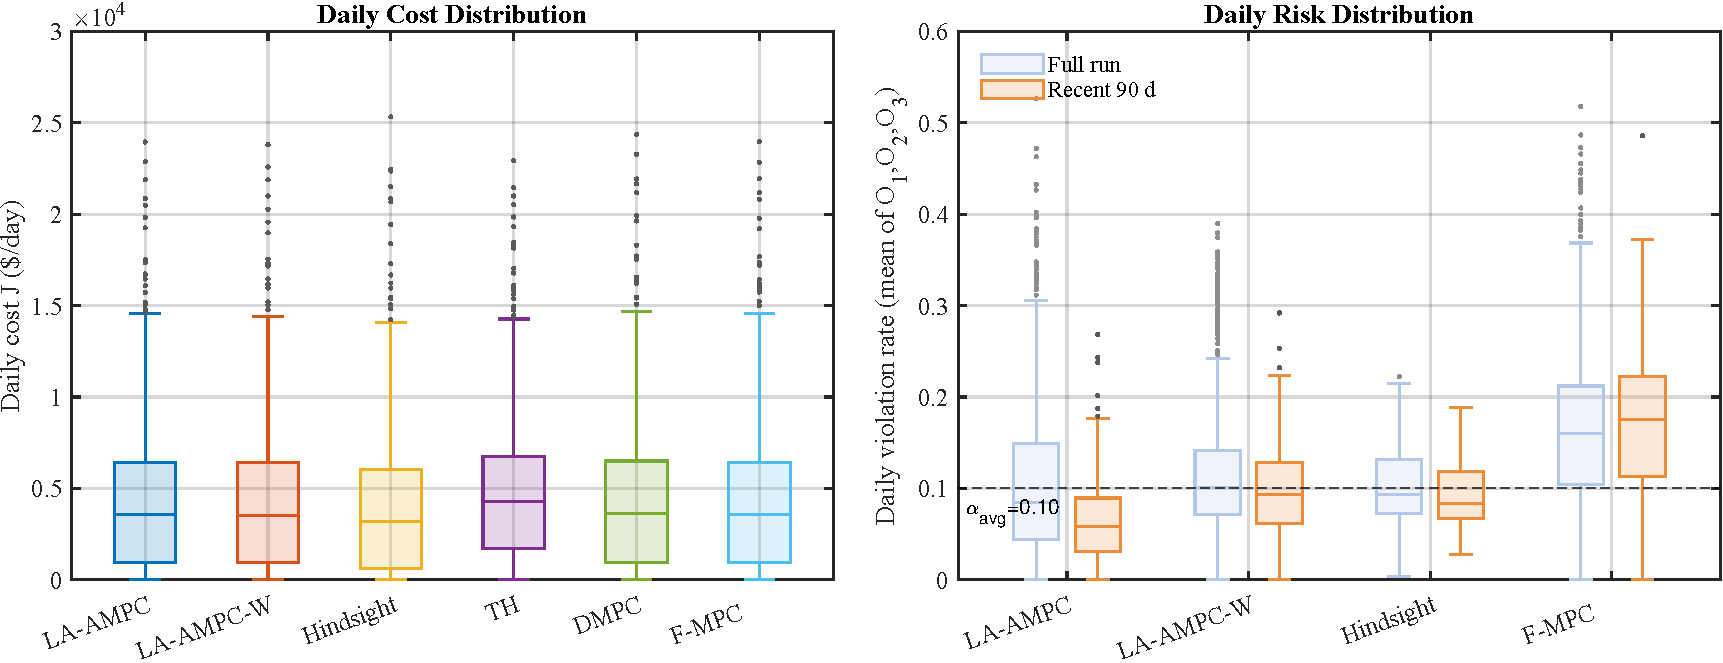
\includegraphics[width=\textwidth,height=0.72\textheight,keepaspectratio]{fig_main_closedloop/fig8_main_daily_distribution_lstm_grouped.pdf}
\caption{Representative daily distributions. Left: full-run daily cost distribution across all methods. Right: daily violation rate distribution (mean of $O_1,O_2,O_3$), comparing the full run and the most recent 90 days.}
\label{fig:main_daily_distribution}
\end{figure*}

Among the causal controllers, TH is the most conservative policy: it yields zero recorded violations but incurs the highest cost and the lowest renewable utilization. F-MPC reduces cost at the expense of substantially increased risk. DMPC eliminates recent ESS-bound violations by enforcing the nominal storage bounds, but its thermal violation rate reaches $19.55\%$, indicating that the deterministic policy concentrates risk in the thermal subsystem instead of adaptively balancing the three state constraints. The proposed windowed method remains in the low-cost regime of MPC-based methods while keeping risk and service quality in a controlled range, which supports its design objective of nonconservative yet risk-aware closed-loop operation.
\subsection{Nonconservativeness and Component-Wise Analysis}
\begin{figure*}[t]
\centering
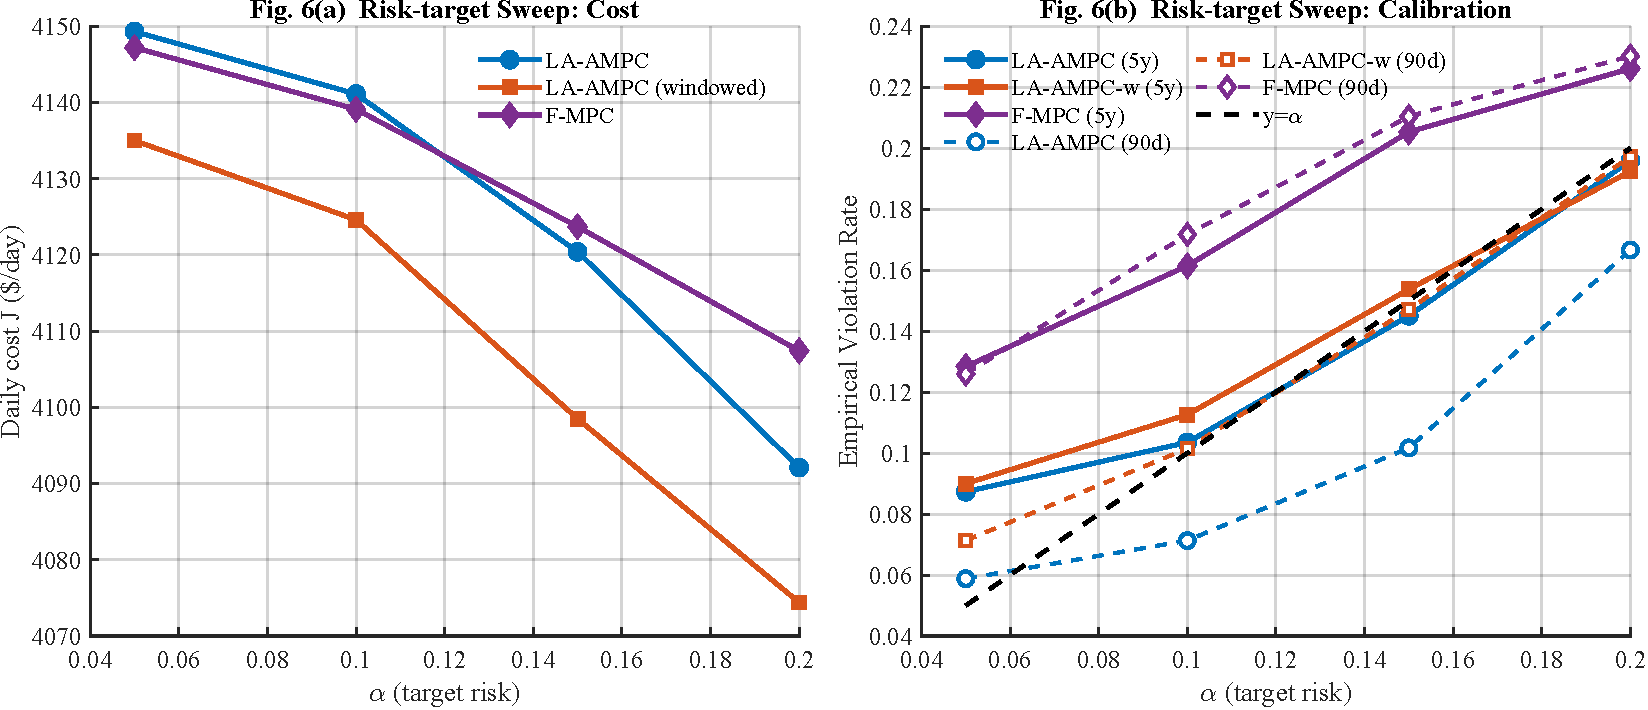
\includegraphics[width=\textwidth,height=0.72\textheight,keepaspectratio]{fig_nonconserv_component/fig9_risk_target_sweep_lstm.pdf}
\caption{Risk-target sweep for nonconservativeness analysis. Solid curves report full 5-year empirical violation rates, dashed curves report recent-90-day rates, and $y=\alpha$ denotes the target line.}
\label{fig:nonconserv_risk_sweep}
\end{figure*}

Nonconservativeness here means economically exploiting the prescribed risk budget rather than systematically under-utilizing it. Fig.~\ref{fig:nonconserv_risk_sweep} and Table~\ref{tab:risk_target_sweep_summary} show the resulting cost-risk frontier: for both LA-AMPC variants, increasing $\alpha$ from $0.05$ to $0.20$ monotonically lowers cost while raising empirical risk. This coupled trend indicates that cost reduction is obtained by adaptive risk-budget use rather than operation at a single conservative point.

The source of this nonconservative behavior is the online adaptive adjustment of the relaxation margins, rather than the static constraint reformulation itself. After re-initializing F-MPC with $\alpha$-dependent initial margins, F-MPC also exhibits monotonic movement with $\alpha$ (Table~\ref{tab:risk_target_sweep_summary}). However, its cost-risk points remain dominated by LA-AMPC (windowed): at every tested $\alpha$, LA-AMPC (windowed) attains both lower daily cost and lower empirical violation rate than F-MPC. Compared with LA-AMPC, F-MPC obtains a slightly lower daily cost at $\alpha=0.05$ and $0.10$, but its empirical violation rate is substantially higher (e.g., $12.84\%$ versus $8.73\%$ at $\alpha=0.05$, $16.14\%$ versus $10.35\%$ at $\alpha=0.10$); the marginal cost reduction is therefore obtained by tolerating clearly more constraint violations rather than by reaching a more efficient operating point. This indicates that initial-margin retuning alone can improve target sensitivity but cannot replace online adaptive correction under evolving disturbances. By comparison, the LA-AMPC variants preserve a more efficient cost-risk frontier and better risk calibration across the full sweep, which is the characteristic behavior expected from an adaptive design.

\begin{table*}[t]
\centering
\caption{Component-wise ablation summary (default vs. no-terminal).}
\label{tab:component_ablation_summary}
\setlength{\tabcolsep}{3pt}
\renewcommand{\arraystretch}{1.05}
\small
\begin{tabular}{llcccc}
\toprule
Method & Setting & \theadcell{Cost $J$\\(\$)} & \theadcell{Risk rate\\(\%)} & \theadcell{SLA\\($\times 10^{-4}$)} & \theadcell{RES\\(\%)} \\
\midrule
\datamulti{LA-AMPC}
& default     & 4141.1 & 10.35 & 0.8452 & 90.48 \\
& no-terminal & 4383.7 & 15.22 & 1.3897 & 88.54 \\
\midrule
\datamulti{LA-AMPC (win.)}
& default     & 4124.6 & 11.26 & 0.8209 & 90.75 \\
& no-terminal & 4369.8 & 15.28 & 1.3890 & 88.79 \\
\bottomrule
\end{tabular}
\vspace{2pt}
\begin{flushleft}
\footnotesize \textit{Note:} Cost $J$ is the average daily operating cost over the full 5-year run and is reported in U.S. dollars per day; risk rate is the full-run (5-year) average empirical violation rate reported in percentage.
\end{flushleft}
\end{table*}

\begin{table*}[t]
\centering
\caption{Risk-target sweep summary.}
\label{tab:risk_target_sweep_summary}
\setlength{\tabcolsep}{4pt}
\renewcommand{\arraystretch}{1.05}
\small
\begin{adjustbox}{max width=\linewidth}
\begin{tabular}{c ccc ccc ccc}
\toprule
\theadmulti{Target\\risk} &
\multicolumn{3}{c}{LA-AMPC} &
\multicolumn{3}{c}{LA-AMPC (windowed)} &
\multicolumn{3}{c}{F-MPC} \\
\cmidrule(lr){2-4}\cmidrule(lr){5-7}\cmidrule(lr){8-10}
& \theadcell{Cost $J$\\(\$)} & \theadcell{Risk\\(\%)} & \theadcell{Recent risk\\(\%)} &
  \theadcell{Cost $J$\\(\$)} & \theadcell{Risk\\(\%)} & \theadcell{Recent risk\\(\%)} &
  \theadcell{Cost $J$\\(\$)} & \theadcell{Risk\\(\%)} & \theadcell{Recent risk\\(\%)} \\
\midrule
0.05 & 4149.3 & 8.73 & 5.88 & 4135.0 & 9.00 & 7.13 & 4147.2 & 12.84 & 12.59 \\
0.10 & 4140.9 & 10.35 & 7.13 & 4124.5 & 11.26 & 10.15 & 4139.1 & 16.14 & 17.17 \\
0.15 & 4120.4 & 14.50 & 10.17 & 4098.5 & 15.37 & 14.71 & 4123.7 & 20.53 & 21.04 \\
0.20 & 4092.1 & 19.59 & 16.66 & 4074.4 & 19.24 & 19.72 & 4107.4 & 22.61 & 23.02 \\
\bottomrule
\end{tabular}
\end{adjustbox}
\vspace{2pt}

\scriptsize \textit{Notes:} Cost $J$ is the average daily operating cost over the full 5-year run and is reported in U.S. dollars per day. ``Risk'' denotes the 5-year full-run average empirical violation rate, while ``Recent Risk'' denotes the empirical violation rate averaged over the most recent 90 days.
\end{table*}

Table~\ref{tab:component_ablation_summary} quantifies the contribution of offline training through the terminal-value component. Removing the terminal value (no-terminal) consistently degrades all key metrics for both controllers. For LA-AMPC, the daily cost increases from $4141.1$ to $4383.7$~\$/day ($+5.86\%$), the risk increases from $10.35\%$ to $15.22\%$, the SLA-unserved ratio increases from $0.8452$ to $1.3897$, and the RES utilization decreases from $90.48\%$ to $88.54\%$. The same pattern is observed for the windowed LA-AMPC. These consistent shifts indicate that the terminal-value term is not an auxiliary regularizer but an essential component that reduces short-horizon suboptimality and stabilizes the cost--risk--service tradeoff over long horizons.

The role of the windowed design is visible in Table~\ref{tab:risk_target_sweep_summary} by comparing LA-AMPC and LA-AMPC (windowed) under the same $\alpha$. The windowed version yields lower cost at all tested risk targets (approximately $0.34\%$--$0.53\%$ relative reduction) while maintaining comparable risk levels. The reason is that the original LA-AMPC tracks the full-history violation rate, so relatively high violations in the early stage can force the later closed-loop operation to remain persistently below the target level $\alpha$, thereby underusing the allowable chance-constraint budget. By contrast, the windowed design tracks the recent violation rate over the most recent horizon, which allows the controller to respond more directly to the current risk level and exploit the feasible set more effectively. The main benefit of the window mechanism is therefore better use of the risk budget and hence lower cost, rather than shifting the controller to a fundamentally different risk regime.
\subsection{Robustness and Sensitivity Analysis}
\begin{figure*}[t]
\centering
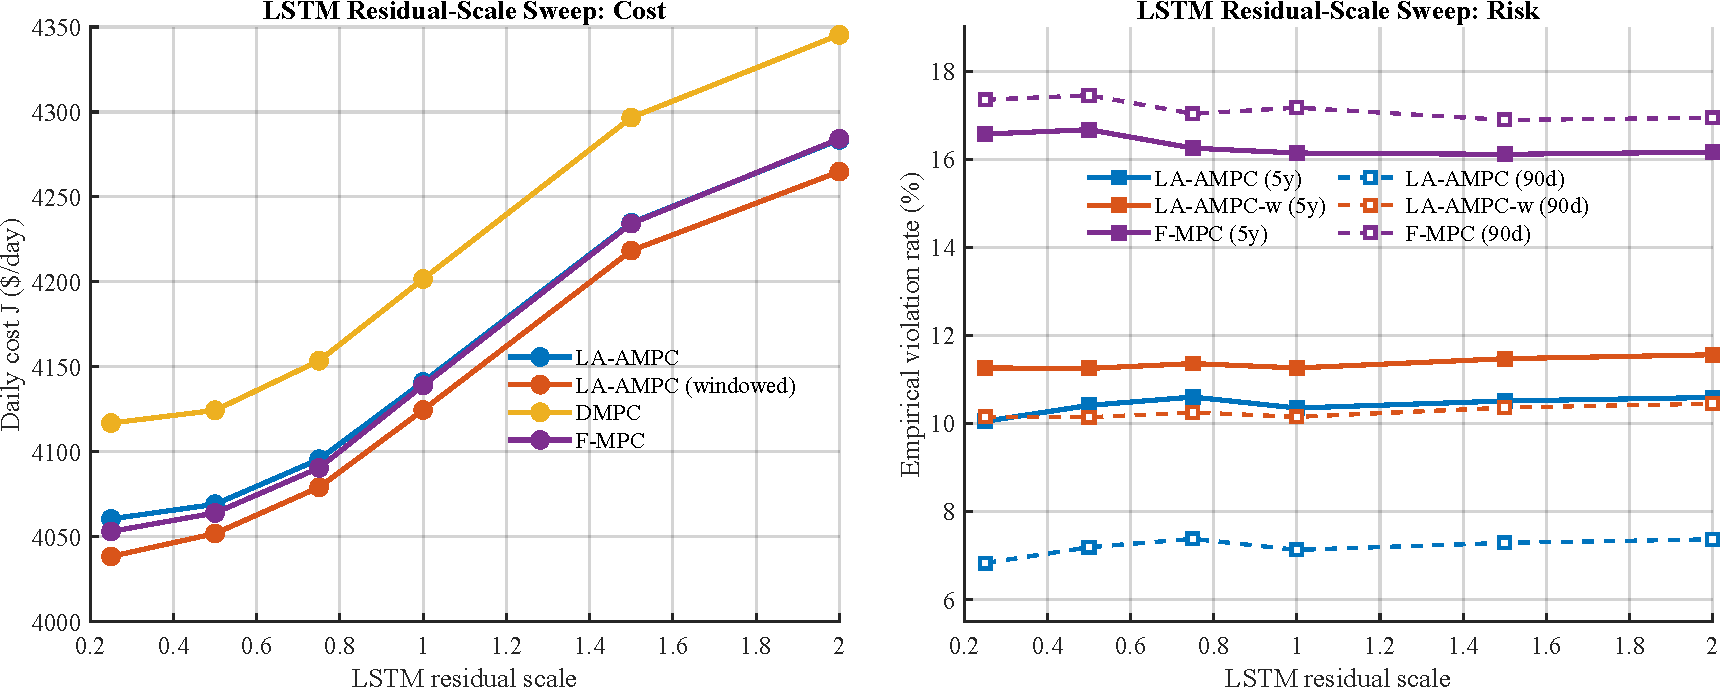
\includegraphics[width=\textwidth,height=0.72\textheight,keepaspectratio]{fig_robustness_sensitivity/fig10_lstm_residual_forecast_sweep.pdf}
\caption{LSTM residual-scale forecast-error sweep: daily cost across methods and empirical violation rates for the chance-constrained controllers.}
\label{fig:robust_forecast_sweep}
\end{figure*}

\input{fig_robustness_sensitivity/tableR1_forecast_sweep.tex}

\begin{figure*}[t]
\centering
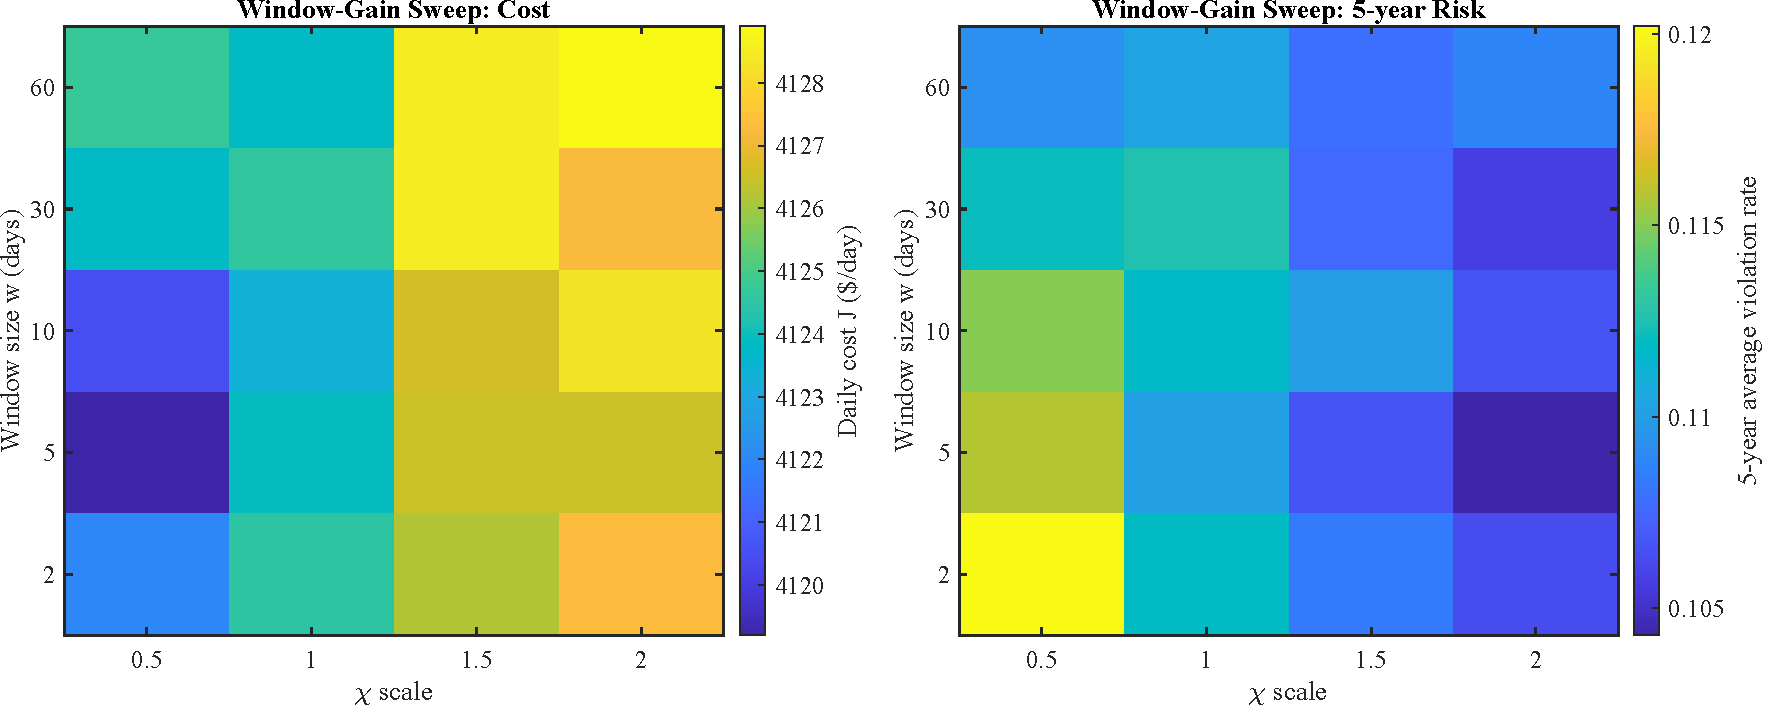
\includegraphics[width=\textwidth,height=0.72\textheight,keepaspectratio]{fig_robustness_sensitivity/fig11_window_gain_sweep_lstm.pdf}
\caption{Window-size and gain-scale sensitivity: heatmaps of daily cost and 5-year average empirical violation rate.}
\label{fig:robust_hyper_sweep}
\end{figure*}

Fig.~\ref{fig:robust_forecast_sweep} and Table~\ref{tab:robust_forecast_sweep} report a residual-based sensitivity test in which the empirical LSTM forecast residuals are scaled from $0.25$ to $2.00$ times their nominal level. Across this range, all optimization-based methods show smooth cost changes without an abrupt regime shift. The proposed LA-AMPC (windowed) maintains the lowest daily cost at every tested residual scale ($4038.4$--$4264.9$~\$/day), while its recent-90-day empirical violation rate remains tightly concentrated around $10.1\%$--$10.5\%$.

The cost advantage of the windowed method is also preserved in the high-residual regime. At residual scale $2.00$, LA-AMPC (windowed) attains a lower daily cost than LA-AMPC ($4264.9$ vs.\ $4283.6$~\$/day, about $0.44\%$ reduction), DMPC ($4345.4$~\$/day, about $1.85\%$ reduction), and F-MPC ($4284.2$~\$/day, about $0.45\%$ reduction). In the risk panel, F-MPC remains at a substantially higher empirical violation level, indicating weaker calibration under residual-amplified forecast errors.

Fig.~\ref{fig:robust_hyper_sweep} further examines hyper-parameter sensitivity over $w\in\{2,5,10,30,60\}$ days and $\chi\in\{0.5,1.0,1.5,2.0\}$. The daily-cost heatmap shows a compact variation range ($4119.2$--$4128.9$~\$/day, about $0.24\%$ spread), while the average risk heatmap remains within a relatively narrow band ($10.4\%$--$12.0\%$). These results show that varying the controller hyper-parameters induces only small changes in either the operating cost or the average empirical risk, supporting the robustness of the proposed method to parameter selection.

Increasing $\chi$ tends to lower the empirical violation rate at the cost of a slightly higher operating cost. For example, at $w=30$ days, increasing $\chi$ from $0.5$ to $2.0$ reduces the average risk from $11.21\%$ to $10.57\%$ while the daily cost increases from $4123.8$ to $4127.2$~\$/day. By contrast, the window length mainly affects the smoothness and noise-rejection property of the adaptive update loop rather than shifting the operating point substantially. Nevertheless, the changes in both cost and empirical risk across the tested window lengths remain limited, indicating low sensitivity to this parameter. The window length can therefore be selected primarily according to practical considerations such as responsiveness and noise rejection.

\section{Conclusion}\label{sec:conclusion}

This paper has developed a learning-assist adaptive MPC framework for single data center energy management under multi-source uncertainty, in which renewable dispatch, storage operation, cooling control, and heterogeneous deferrable workloads are coordinated within a single closed-loop optimization architecture. The proposed design combines an offline-trained DP-inspired terminal value function with a sliding-window adaptive chance-constraint relaxation mechanism, and further introduces a windowed violation rate estimator to improve responsiveness to recent risk dynamics. Consequently, the controller preserves explicit physical and service-level constraints while alleviating the conservatism of fixed-margin control. In closed-loop simulations, the proposed method attained a better calibrated cost--risk--service tradeoff than deterministic MPC, fixed-relaxation MPC, and threshold-based control. Among causal controllers, the windowed variant achieved the smallest cost gap to the hindsight benchmark, the lowest SLA-unserved ratio, and the highest renewable-utilization ratio.

Together with the structural performance characterization of the windowed update, these results support the use of empirical risk tracking over a recent window for nonconservative closed-loop operation. The case studies also identified the mechanisms underlying these gains. The risk-target sweep showed that adaptive relaxation can move the operating point along a practical cost-risk frontier rather than remaining at an over-conservative operating point, and the windowed design improves risk-budget utilization by reacting to recent rather than full-history violations. Component-wise ablation confirmed that the terminal-value term is essential for mitigating short-horizon suboptimality, since removing it simultaneously degrades cost, risk, and SLA performance. Robustness studies under forecast-error and hyper-parameter perturbations further showed that both operating cost and empirical risk vary only mildly across the tested settings, demonstrating the practical applicability of the proposed method under forecast and parameter perturbations.

% TODO: Add actual acknowledgements and verified funding information if applicable.
% IEEE template instructions have been removed.

\FloatBarrier
\appendix
\section{Offline-Training Equivalence}\label{app:offline_training_proof}
\subsection{Uncertainty Discretization and Histogram Construction}
The offline approximation replaces the original uncertainty
$\xi_t=\{\gamma_t,\omega_t^r,c_t^I,C_{t,k}^D\}$ by the reduced variable
$\xi_t'=\{\gamma_t,\omega_t^r,p_t^{\text{DC}}\}$, where $p_t^{\text{DC}}$ is defined in \eqref{eq:pdc}. Historical
samples of $(\gamma_t,\omega_t^r,p_t^{\text{DC}})$ are then binned to construct a finite scenario set
$\{\xi^{\prime(l)}\}_{l=1}^{N_{\xi'}}$ with empirical probabilities $\{\rho_l\}_{l=1}^{N_{\xi'}}$.

Specifically, the renewable power range $[0,P_{\text{cap}}^R]$ is partitioned into $N_R$ intervals
$\{\Omega_i^R\}_{i=1}^{N_R}$, and the data center total power range $[0,P_{\max}^L]$ is partitioned into
$N_L$ intervals $\{\Omega_j^L\}_{j=1}^{N_L}$ so that the sample counts are approximately balanced across bins.
Representative values $\{\omega_i^r\}$ and $\{p_j^{\text{DC}}\}$ are taken as the interval midpoints.

For electricity price, the real line is partitioned into $N_\gamma$ intervals
$\{\Omega_k^\gamma\}_{k=1}^{N_\gamma}$, with the first and last intervals left- and right-unbounded, respectively.
The endpoint representatives are set to the historical extrema $\gamma_{\min}$ and $\gamma_{\max}$, while the remaining
representatives $\{\gamma^{(k)}\}$ are chosen as interval midpoints.

The Cartesian product of these one-dimensional partitions induces
$N_{\xi'}=N_R N_L N_\gamma$ multivariate cells
$\Omega_l^{\xi'}=\Omega_i^R\times\Omega_j^L\times\Omega_k^\gamma$.
For each cell, the representative scenario is
$\xi^{\prime(l)}=[\omega^{(i)},p_{\text{DC}}^{(j)},\gamma^{(k)}]^\top$,
and the empirical probability $\rho_l$ is estimated by the sample frequency of that cell.

\subsection{Feasible Successor Index Set}\label{subsec:successor_set}
For a feasible transition from $x_t=x^{(m)}$ to $x_{t+1}=x^{(n)}$, the corresponding ESS and renewable dispatch are
\begin{equation}\label{ttmp1}
\left\{\begin{array}{l}
\text{If } x_{t+1}\ge x_t:
p_t^{{bs}} = p_t^{\text{ch}}=\dfrac{x_{t+1}-x_t}{\eta_{\text{ch}}\Delta\tau}, \quad p_t^{\text{dis}} = 0,\\[2mm]
\text{If } x_{t+1}< x_t:
p_t^{\text{ch}} = 0, p_t^{\text{dis}}=-\dfrac{(x_{t+1}-x_t)\,\eta_{\text{dis}}}{\Delta\tau},\\[2mm]
p_t^r=\min \left\{\omega_t^r,\ p_t^{bs}+p_t^{\text{DC}}\right\}.
\end{array}\right.
\end{equation}
Because $p_t^{\text{DC}}=p_t^{\text{ser}}+p_t^{\text{cool }}$ is fixed by the reduced uncertainty sample $\xi^{\prime(l)}$, the grid power is obtained from the power-balance relation
\begin{equation}\label{ttmp2}
p_t^{gd} + p_t^r=p_t^{bs}+p_t^{\text{DC}}.
\end{equation}
Thus, for each triple $(m,n,l)$, the dispatch variables can be predetermined, and the feasible successor set depends only on the bounds of $p_{m,n,l}^{bs}$:
\begin{align*}
\overline{p}^{bs}_{m,n,l}
&= \min\!\left\{\begin{aligned}&P_{\max}^{bs},\ P_{\max}^{gd}+\omega_r^{(l)}-p^{(l)}_{\text{DC}},\\&\frac{E_{\max}^{bs}-x^{(m)}}{\eta_{\text{ch}}\Delta\tau}\end{aligned}\right\},\\
\underline{p}^{bs}_{m,n,l}
&= \max\!\left\{\begin{aligned}&-P_{\max}^{bs},\ -p^{(l)}_{\text{DC}},\\&\frac{(E_{\min}^{bs}-x^{(m)})\,\eta_{\text{dis}}}{\Delta\tau}\end{aligned}\right\}.
\end{align*}
These bounds induce the successor-state interval
\begin{align*}
\overline{x^{(n)}} &= x^{(m)} + \eta_{\text{ch}}\,\overline{p}^{bs}_{m,n,l}\, \Delta \tau, \\
\underline{x^{(n)}} &= x^{(m)} + \frac{1}{\eta_{\text{dis}}}\,\underline{p}^{bs}_{m,n,l}\, \Delta \tau,
\end{align*}
and hence the discrete feasible index set
\begin{equation}\label{temp5}
U_n(m,l) := \{0,1, \cdots, M\} \cap[\underline{n}, \bar{n}],
\end{equation}
where $\bar{n}=\left\lfloor\frac{\overline{x^{(n)}}}{E_{\max }^{bs}-E_{\min }^{bs}}\right\rfloor$ and $\underline{n}=\left\lceil\frac{\underline{x^{(n)}}}{E_{\max }^{bs}-E_{\min }^{bs}}\right\rceil$, with $\lfloor \cdot \rfloor$ and $\lceil \cdot \rceil$ denoting the floor and ceiling operators, respectively.

\subsection{Bellman-Equation Construction}
The offline objective is the infinite-horizon discounted operating cost of the reduced surrogate
$\min_{\{e_\tau^u\}} \mathbb{E}\big[\sum_{\tau=t_0}^{\infty} \beta^{\tau-t_0}\gamma_\tau p_\tau^{gd}\Delta\tau\big]$,
with storage transition $x_{t+1}=f(x_t,e_t^u):=x_t+\Delta\tau\big(\eta_{\text{ch}} p_t^{\text{ch}}-p_t^{\text{dis}}/\eta_{\text{dis}}\big)$ and feasible set $U(x_t,\xi_t)$.
In the reduced surrogate, successive scenarios are independent across time and have the fixed joint empirical distribution specified above. This is a modeling approximation; stationarity of the observed process alone would not justify replacing conditional future distributions by a common marginal distribution. Applying the Bellman principle for discounted MDPs in Section~6.2 of~\cite{puterman1994_mdp_book}, let $W(x,\xi)$ denote the value after observing the current scenario, while $V(x)$ denotes the value before observing it. Then
\[
\begin{aligned}
W(x,\xi)&=\min_{e^u\in U(x,\xi)}\big\{\gamma(\xi)p^{gd}(e^u)\Delta\tau\\
&\qquad\qquad +\beta V(f(x,e^u))\big\},\\
V(x)&=\mathbb{E}^{\xi}[W(x,\xi)].
\end{aligned}
\]
The continuation value depends only on the successor storage state because the next scenario has the same distribution independently of the current scenario and action. Substituting the first relation into the second gives~\eqref{eq:bellman_stationary}. For the discrete construction, write $V_m=V(x^{(m)})$, $W_m(l)=W(x^{(m)},\xi^{\prime(l)})$, and $c_{mnl}=\gamma^{(l)}p_{m,n,l}^{gd}\Delta\tau$. The same relations become
\[
\begin{aligned}
W_m(l)&=\min_{n\in U_n(m,l)}\{c_{mnl}+\beta V_n\},\\
V_m&=\sum_l\rho_l W_m(l),
\end{aligned}
\]
which yield~\eqref{temp4}. The weighted scenario sums are evaluated directly; random sampling during the LP solve is not required.

\subsection{Mapping between LP Variables and Value Function}
At the optimum $(\{z_m^{\mathrm{LP}}\},\{s_{m,l}^{\mathrm{LP}}\})$ of \eqref{object train}--\eqref{line2 train}, the LP variables encode the discretized value function as follows: $z_m^{\mathrm{LP}}=V(x^{(m)})$ is the value at storage grid point $m$, and
\begin{equation*}
s_{m,l}^{\mathrm{LP}}=\min_{n\in U_n(m,l)}\big\{\gamma^{(l)}p_{m,n,l}^{gd}\Delta\tau+\beta\, z_n^{\mathrm{LP}}\big\}
\end{equation*}
is the inner conditional cost-to-go under scenario $\xi^{\prime(l)}$. Constraint~\eqref{line1 train} encodes the outer expectation $V(x^{(m)})=\sum_l \rho_l s_{m,l}$, and \eqref{line2 train} encodes the inner Bellman minimization over feasible successor indices $n\in U_n(m,l)$. For the discretized surrogate MDP, the bidirectional equivalence between \eqref{temp4} and \eqref{object train}--\eqref{line2 train} is a direct specialization of the standard LP formulation of finite-state discounted MDPs discussed in Section~6.9 of~\cite{puterman1994_mdp_book}; the binding-constraint argument is omitted. The continuous terminal value $V(x_t)$ is then obtained from $V(x^{(m)})=z_m^{\mathrm{LP}}$ for $m=0,\ldots,M$ by piecewise-linear interpolation, yielding the convex nonincreasing profile visualized in Fig.~\ref{fig:offline_value}.

\section{Convergence of the Windowed Update}\label{app:adaptive_mpc_proof}

\subsection{Detailed Statement and Proof of Theorem~\ref{thm:window_conv}}\label{subsec:thm-proof}
\noindent\textbf{Detailed statement of Theorem~\ref{thm:window_conv}.}
Given $\alpha_i \in (0,1)$, the ideal surrogate $Z_t^{i,w,*}$ is monotonically decreasing for all $t \ge t_0$ whenever the ideal control policy is applied, where
\begin{equation}\label{ideal p}
p_{t+1}^{i,*} :=
\begin{cases}
1, & \alpha_i - Y_{t}^{i,w} + \dfrac{2O^{i}_{t-w+1}-1}{2w} > 0,\\[2mm]
0, & \alpha_i - Y_{t}^{i,w} + \dfrac{2O^{i}_{t-w+1}-1}{2w} < 0.
\end{cases}
\end{equation}
Moreover, $Z_t^{i,w,*}$ converges to
\begin{equation}\label{minimum Z}
    Z_{\min}^{i,w,*} = \min_{k \in \{0, 1, 2, \dots, w\}} \left| \alpha_i - \frac{k}{w} \right|.
\end{equation}

\begin{proof}
\textit{Step 1: boundedness and one-step drift expression.} Since $O_t^i \in \{0,1\}$, $Y_t^{i,w} \in [0,1]$, and $\alpha_i \in (0,1)$, we have $Z_t^{i,w} = \vert \alpha_i - Y_t^{i,w} \vert \in [0,1)$. Hence $\mathbb{E}\left[Z_t^{i,w}\right] < \infty$.

Rewrite \eqref{New Y} as
\begin{equation} \label{New Y t+1}
    Y_{t+1}^{i,w} = Y_{t}^{i,w} + \frac{O_{t+1}^i - O_{t-w+1}^i}{w}.
\end{equation}
Define the conditional drift
\begin{equation}\label{temp eq1}
\begin{aligned}\Delta_t^{i,w}
&:= \mathbb{E}\!\left[
\left|\alpha_i - Y_t^{i,w} - \frac{O_{t+1}^i - O_{t-w+1}^i}{w}\right|
\middle| \mathcal{F}_t
\right]
\\ &\quad-\left|\alpha_i-Y_t^{i,w}\right|.
\end{aligned}
\end{equation}
Using $p_{t+1}^i=P(O_{t+1}^i=1\mid\mathcal{F}_t)$, \eqref{temp eq1} becomes
\begin{equation} \label{Delta i}
    \Delta_t^{i,w}
    = p_{t+1}^i \varphi_{t}^i + \left[
    \left|\alpha_i - Y_t^{i,w} + \frac{O_{t-w+1}^i}{w}\right|
    - \left|\alpha_i - Y_t^{i,w} \right|
    \right],
\end{equation}
where
\begin{equation}\label{varphi i}
    \varphi_{t}^i =
    \left|\alpha_i - Y_t^{i,w} + \frac{O_{t-w+1}^i-1}{w} \right|
    -\left|\alpha_i - Y_t^{i,w} + \frac{O_{t-w+1}^i}{w} \right|.
\end{equation}

\textit{Step 2: monotone decrease under the ideal policy.} We next show that $\Delta_t^{i,w,*}\le 0$ when the ideal policy \eqref{ideal p} is applied.

\textbf{Case 1.}
\begin{equation}\label{temp eq2}
    \varphi_t^i < 0 \Leftrightarrow Y_{t}^{i,w} < \alpha_i + \dfrac{2O^{i}_{t-w+1}-1}{2w}
    \Rightarrow p_{t+1}^{i,*} = 1.
\end{equation}
Suppose, for contradiction, that $\Delta_t^{i,w,*} > 0$ under $p_{t+1}^{i,*} = 1$. Then
\begin{equation}\label{temp eq3}
    Y_t^{i,w} > \alpha_i + \frac{O_{t-w+1}^i-1}{2w} \text{ and } O_{t-w+1}^i \neq 1.
\end{equation}
Because $O_{t-w+1}^i \in \{0,1\}$, this forces $O_{t-w+1}^i = 0$, which is incompatible with simultaneously satisfying \eqref{temp eq2} and \eqref{temp eq3}. Hence $\Delta_t^{i,w,*} \leq 0$.

\textbf{Case 2.}
\begin{equation}\label{temp eq4}
    \varphi_t^i > 0 \Leftrightarrow Y_{t}^{i,w} > \alpha_i + \dfrac{2O^{i}_{t-w+1}-1}{2w}
    \Rightarrow p_{t+1}^{i,*} = 0.
\end{equation}
Suppose, for contradiction, that $\Delta_t^{i,w,*} > 0$ under $p_{t+1}^{i,*} = 0$. Then
\begin{equation}\label{temp eq5}
    Y_t^{i,w} < \alpha_i + \frac{O_{t-w+1}^i}{2w} \text{ and } O_{t-w+1}^i \neq 0.
\end{equation}
This forces $O_{t-w+1}^i = 1$, which cannot coexist with \eqref{temp eq4} and \eqref{temp eq5}. Therefore $\Delta_t^{i,w,*} \leq 0$.

\textbf{Case 3.}
\begin{equation*}
    \varphi_t^i = 0 \Leftrightarrow Y_{t}^{i,w} = \alpha_i + \dfrac{2O^{i}_{t-w+1}-1}{2w}.
\end{equation*}
In this case,
\[
\Delta_t^{i,w,*} = \frac{1}{2w} - \left|\frac{1-2O_{t-w+1}^i}{2w}\right| = 0.
\]

Therefore $Z_{t+1}^{i,w,*}\le Z_t^{i,w,*}$ for all $t\ge t_0$. Since $0\le Z_t^{i,w,*}\le 1$, the monotone convergence theorem implies
\begin{equation*}
    \lim_{t \to \infty} Z_t^{i,w,*} = \inf_{t \ge t_0} Z_t^{i,w,*}.
\end{equation*}

\textit{Step 3: convergence to the minimum quantized error.} We next show that the limit above equals the theoretical minimum in \eqref{minimum Z}. First consider the case without Case 3, namely
\begin{equation} \label{temp eq7}
    Y_{t}^{i,w} \neq \alpha_i + \dfrac{2O^{i}_{t-w+1}-1}{2w}.
\end{equation}
Substituting \eqref{New Y} into \eqref{temp eq7} yields
\[
\alpha_i \neq \frac{2\sum_{\tau = t-w+2}^{t}O_{\tau}^i+1}{2w}.
\]
Hence, if $\alpha_i \neq \frac{2\mathbb{N}+1}{2w}$ for any non-negative integer $\mathbb{N}$, then Case 3 never occurs. Define
\begin{equation*}
    \kappa(\alpha_i,w):=\left(\alpha_i - \frac{1}{2w},\alpha_i + \frac{1}{2w}\right).
\end{equation*}

\begin{lemma}
For some initial time $t_0$, if $Y_{t_0}^{i,w} \in \kappa(\alpha_i,w)$, then $Y_t^{i,w} \in \kappa(\alpha_i,w)$ for all $t > t_0$ under the ideal control policy \eqref{ideal p}.
\end{lemma}
\begin{proof}
If $O_{t-w+1}^{i} = 1$, substituting into \eqref{Delta i} and \eqref{varphi i} gives $\Delta_{t}^{i,w,*} = 0$, so $Y_{t+1}^{i,w} = Y_{t}^{i,w}$. The same conclusion holds when $O_{t-w+1}^{i} = 0$. Thus the interval $\kappa(\alpha_i,w)$ is forward invariant under the ideal policy.
\end{proof}

\begin{lemma}
For some initial time $t_0$, if $Y_{t_0}^{i,w} \notin \kappa(\alpha_i,w)$, then there exists $t' > t_0$ such that $Y_{t'}^{i,w} \in \kappa(\alpha_i,w)$ under the ideal control policy \eqref{ideal p}.
\end{lemma}
\begin{proof}
Assume without loss of generality that $Y_{t_0}^{i,w} \ge \alpha_i + \frac{1}{2w} > 0$. Then there exists at least one $t_1 \in (t_0, t_0 + w - 1)$ such that $O_{t_1 - w + 1}^{i} = 1$. Substituting into \eqref{Delta i} and \eqref{varphi i} yields $\Delta_{t_1}^{i,w,*} < 0$, so the distance to $\alpha_i$ strictly decreases. The case $Y_{t_0}^{i,w} \le \alpha_i - \frac{1}{2w} < 1$ follows analogously.
\end{proof}

By the two lemmas, for any $\alpha_i \in (0,1)$ with $\alpha_i \neq \frac{2\mathbb{N}+1}{2w}$, the ideal-policy trajectory enters and remains in
\begin{equation*}
    \kappa(\alpha_i,w) \cap \left\{0,\tfrac{1}{w},\tfrac{2}{w},\dots,1\right\}.
\end{equation*}
Therefore, $Z_t^{i,w,*}$ converges to the smallest distance between $\alpha_i$ and the quantized grid $\{0,\tfrac{1}{w},\ldots,1\}$, namely $Z_{\min}^{i,w,*}$ in \eqref{minimum Z}.

If $\alpha_i \in \frac{2\mathbb{N}+1}{2w}$, then $Y_t^{i,w}$ eventually oscillates within the two-point set $\left\{\alpha_i - \tfrac{1}{2w},\, \alpha_i + \tfrac{1}{2w}\right\}$. Even in this boundary case, the achieved absolute deviation still equals the theoretical minimum value $Z_{\min}^{i,w,*}$. This completes the proof.
\end{proof}

\subsection{Analysis under the Weaker Attainability Assumption}\label{subsec:weak}

The proof above relies on Assumption~1, which is an oracle-type condition. This subsection establishes Propositions~\ref{prop:onestep}--\ref{prop:upper} stated in Section~\ref{subsec:adaptive_adjustment}, which characterize attainable behavior under the weaker Assumption~\ref{asm:attain}.

\noindent\textbf{Symbol convention.} Throughout this subsection, $\alpha_i^\star=\mathrm{proj}_{[\underline p^i,\overline p^i]}(\alpha_i)$, $\tilde Z_t^{i,w}:=|Y_t^{i,w}-\alpha_i^\star|$, and
\begin{align*}
\varphi_t^\star &:= \big|\alpha_i^\star-Y_t^{i,w}+\tfrac{O_{t-w+1}^i-1}{w}\big|\\&\quad-\big|\alpha_i^\star-Y_t^{i,w}+\tfrac{O_{t-w+1}^i}{w}\big|,\\
c_t^\star &:= \big|\alpha_i^\star-Y_t^{i,w}+\tfrac{O_{t-w+1}^i}{w}\big|-\big|\alpha_i^\star-Y_t^{i,w}\big|.
\end{align*}
Both $\varphi_t^\star$ and $c_t^\star$ are $\mathcal{F}_t$-measurable. By the triangle inequality, $|\varphi_t^\star|\le 1/w$ and $|c_t^\star|\le 1/w$.

\subsubsection{Affine one-step drift}
Define the conditional one-step drift in the projected error:
\begin{equation*}
\Delta_t(p):=\mathbb{E}\!\left[\tilde Z_{t+1}^{i,w}\,\middle|\,\mathcal{F}_t,\,p_{t+1}^i=p\right]-\tilde Z_t^{i,w}.
\end{equation*}

\begin{lemma}[Affine drift]\label{lem:affine}
For any $p\in[0,1]$,
\begin{equation}\label{eq:affine-drift}
\Delta_t(p)=p\,\varphi_t^\star+c_t^\star.
\end{equation}
\end{lemma}

\begin{proof}
The windowed recursion gives $Y_{t+1}^{i,w}=Y_t^{i,w}+(O_{t+1}^i-O_{t-w+1}^i)/w$. Conditioned on $\mathcal{F}_t$, $O_{t+1}^i\sim\mathrm{Bern}(p)$ while $O_{t-w+1}^i$ is $\mathcal{F}_t$-measurable. Hence
\begin{align*}
\mathbb{E}\!\left[\tilde Z_{t+1}^{i,w}\,\middle|\,\mathcal{F}_t\right]
&=p\big|\alpha_i^\star-Y_t^{i,w}+\tfrac{O_{t-w+1}^i-1}{w}\big|\\
&\quad+(1-p)\big|\alpha_i^\star-Y_t^{i,w}+\tfrac{O_{t-w+1}^i}{w}\big|.
\end{align*}
Subtracting $\tilde Z_t^{i,w}=|\alpha_i^\star-Y_t^{i,w}|$ and regrouping yields $\Delta_t(p)=p\varphi_t^\star+c_t^\star$.
\end{proof}

\subsubsection{Proof of Proposition~\ref{prop:onestep} (one-step optimality)}

Because $\Delta_t(p)$ is affine in $p$, its minimum over the compact interval $[\underline p^i,\overline p^i]$ is attained at an endpoint determined by the sign of $\varphi_t^\star$:
\begin{equation*}
\arg\min_{p\in[\underline p^i,\overline p^i]}\Delta_t(p)=
\begin{cases}
\{\overline p^i\}, & \varphi_t^\star<0,\\
\{\underline p^i\}, & \varphi_t^\star>0,\\
[\underline p^i,\overline p^i], & \varphi_t^\star=0.
\end{cases}
\end{equation*}
The extreme-point selection rule that picks $\overline p^i$ when $\varphi_t^\star<0$ and $\underline p^i$ when $\varphi_t^\star>0$ therefore realizes the conditional argmin of $\mathbb{E}[|Y_{t+1}^{i,w}-\alpha_i^\star|\,|\,\mathcal{F}_t]$. The update rule \eqref{update h new} preserves this sign structure because the bracketed term $\alpha_i-Y_t^{i,w}+(2O_{t-w+1}^i-1)/(2w)$ shares the sign of $-\varphi_t^\star$ up to the projection effect $\alpha_i\mapsto\alpha_i^\star$.\hfill$\blacksquare$

\subsubsection{Proof of Proposition~\ref{prop:lower} (structural lower bound)}

Let $\rho^\star$ be any stationary distribution induced by a policy with $p_t^i\in[\underline p^i,\overline p^i]$ a.s.. Stationarity and the tower rule give
\begin{equation*}
\mathbb{E}_{\rho^\star}[Y_t^{i,w}]
=\tfrac{1}{w}\sum_{\tau=t-w+1}^{t}\mathbb{E}_{\rho^\star}[O_\tau^i]
=\mathbb{E}_{\rho^\star}[p_t^i],
\end{equation*}
which lies in $[\underline p^i,\overline p^i]$. Jensen's inequality then yields
\begin{equation*}
\begin{aligned}\mathbb{E}_{\rho^\star}|Y_t^{i,w}-\alpha_i|
&\ge \big|\mathbb{E}_{\rho^\star}[Y_t^{i,w}]-\alpha_i\big|
\\ &\ge \inf_{p\in[\underline p^i,\overline p^i]}|p-\alpha_i|
= |\alpha_i-\alpha_i^\star|,\end{aligned}
\end{equation*}
where the last equality follows from the definition of the projection.\hfill$\blacksquare$

\subsubsection{Proof of Proposition~\ref{prop:upper} (constructive upper bound)}

Consider the constant policy $\pi^c$ defined by $p_t^i\equiv\alpha_i^\star$. Since $\alpha_i^\star\in[\underline p^i,\overline p^i]\subseteq\mathcal{P}_t$ for all $t$, $\pi^c$ is feasible under Assumption~\ref{asm:attain}.

Under $\pi^c$, the sequence $\{O_\tau^i\}_{\tau\ge t_0}$ is i.i.d.\ $\mathrm{Bern}(\alpha_i^\star)$. The windowed average $Y_t^{i,w}=(1/w)\sum_{\tau=t-w+1}^{t}O_\tau^i$ therefore satisfies
\begin{equation*}
\mathbb{E}[Y_t^{i,w}]=\alpha_i^\star,\qquad
\mathrm{Var}[Y_t^{i,w}]=\tfrac{\alpha_i^\star(1-\alpha_i^\star)}{w}\le\tfrac{1}{4w}.
\end{equation*}
By Cauchy--Schwarz,
\begin{equation*}
\mathbb{E}|Y_t^{i,w}-\alpha_i^\star|
\le \sqrt{\mathrm{Var}[Y_t^{i,w}]}
\le\tfrac{1}{2\sqrt{w}}.
\end{equation*}
Triangle inequality with the projection gap gives
\begin{equation*}
\mathbb{E}|Y_t^{i,w}-\alpha_i|
\le |\alpha_i-\alpha_i^\star|+\mathbb{E}|Y_t^{i,w}-\alpha_i^\star|
\le |\alpha_i-\alpha_i^\star|+\tfrac{1}{2\sqrt{w}}.
\end{equation*}
The concentration bound follows from Hoeffding's inequality applied to the bounded i.i.d.\ sum $\sum_{\tau}O_\tau^i$.\hfill$\blacksquare$

\subsubsection{Relation to Theorem~\ref{thm:window_conv}}
Propositions~\ref{prop:onestep}--\ref{prop:upper} and Theorem~\ref{thm:window_conv} characterize complementary aspects of the windowed mechanism:
\begin{itemize}
\item Theorem~\ref{thm:window_conv} (under Assumption~1) gives a pathwise convergence statement on the quantized grid for the oracle-driven trajectory.
\item Propositions~\ref{prop:onestep}--\ref{prop:upper} (under Assumption~\ref{asm:attain}) give an attainable performance envelope $|\alpha_i-\alpha_i^\star|+\mathcal{O}(1/\sqrt{w})$ that does not rely on oracle-level controllability.
\end{itemize}
Together, the two analyses bracket the achievable behavior: the oracle case (Theorem~\ref{thm:window_conv}) is the best case where the projection gap vanishes ($\alpha_i^\star=\alpha_i$ whenever $[\underline p^i,\overline p^i]=[0,1]$), and Proposition~\ref{prop:lower} provides the structural floor for the non-oracle case. The empirical results in Section~\ref{sec:case_studies} fall comfortably within this envelope.



\FloatBarrier
\bibliographystyle{energy-buildings-num}
\bibliography{references}

\end{document}
